\documentclass{revtex4-2}
\usepackage{amsmath}
\usepackage{booktabs}
\usepackage{amsmath, amssymb, amsthm}
\usepackage{geometry}
\usepackage{graphicx}
\usepackage{tikz}
\usepackage{booktabs}
\usepackage{hyperref}
\usepackage{fontspec}
\setmainfont{Segoe UI This}

\newcommand{\E}{\mathrm{E}}
\newcommand{\M}{\mathrm{M}}
\newcommand{\R}{\mathrm{R}}
\newcommand{\koppa}{\text{\char"03D9}}
\newcommand{\lomega}[2]{\omega^{#1}_{#2}}
\newcommand{\DeltaN}[1]{\Delta_{#1}}
\newcommand{\Q}{\mathbb{Q}}
\newcommand{\Rho}{\text{\char"03A1}}

\geometry{margin=.4in}

\newtheorem{theorem}{Theorem}[section]
\newtheorem{lemma}[theorem]{Lemma}
\newtheorem{definition}[theorem]{Definition}
\newtheorem{corollary}[theorem]{Corollary}
\newtheorem{proposition}[theorem]{Proposition}

\begin{document}

\title{Triadic Rational Dynamics and Convergence to Quadratic Irrationals: A Structural Analysis of Unreduced Oscillations}
\author{D. Veneziano}
\date{January 5, 2026}

\newpage 
\tableofcontents
\newpage

\begin{abstract}
We present a unified framework for constructing discrete dynamical systems on the domain of unreduced integer pairs that converge to quadratic irrational attractors. By rejecting the axiom of simplification (GCD reduction) and operating strictly via mediant addition and transformative reciprocal swaps, we define a class of triadic cycles that exhibit stable oscillatory convergence. We derive the governing transition matrices, perform a full spectral analysis to prove convergence to limits such as $\sqrt{2}$ and the Silver Ratio $\delta_S$, and establish that these irrational constants emerge as the time-averaged barycenters of deterministic rational orbits. Furthermore, we analyze the structural growth of the system, demonstrating that the logarithm of the denominator grows linearly with the number of cycles, establishing a direct relationship between structural entropy and numerical precision.
\end{abstract}

\maketitle

\section{Introduction: The Mask Postulate and Rational Oscillation}

The approximation of irrational numbers is traditionally approached through the lens of real analysis, where rational sequences are viewed as imperfect approximations converging to a static truth. Classical methods, such as continued fractions and Newton's method, typically operate in the field of real numbers and require division, reduction to lowest terms, or advanced analysis. In this manuscript, we explore a contrasting paradigm: discrete dynamical systems defined on unreduced integer pairs. We construct systems using only simple operations---coordinate addition and coordinate swapping---applied in periodic cycles. Despite their simplicity, these systems exhibit rich spectral behavior and converge to irrational limits in structured, oscillatory patterns.

Our core philosophical stance, derived from the Axiom of Structural Integrity, posits that irrational constants are not ontological primitives. Instead, they are phenomenological masks---statistical artifacts of high-frequency rational oscillation. The mathematical limit is merely a low-resolution observation of this mechanism. The true physical value of a system is the active oscillating sequence of integer pairs. Our goals are twofold: first, to analyze, classify, and extend triadic systems that converge to specific quadratic irrational numbers; second, to develop a general constructive method applicable to any quadratic irrational $\alpha$ satisfying $\alpha^2 - T\alpha + D = 0$. We show that every such irrational limit arises from an appropriate product of elementary integer operations acting on unreduced rational pairs.

The exposition is intentionally meticulous. In Section 2, we formalize the notion of unreduced rational pairs and mediant ordering. Section 3 introduces the triadic update cycle and derives its matrix representation. Section 4 provides a complete spectral analysis of the induced matrix dynamics, while Section 5 supplies a constructive convergence proof using nested mediant intervals. Section 6 establishes the alternating convergence pattern. Section 8 introduces the extended cycle for the Silver Ratio, and Section 10 analyzes the structural entropy of the system.

\section{Understanding the Matrix-Eigenvalue-Irrational Connection}

This section provides a comprehensive explanation of how integer matrices, eigenvalues, 
and quadratic irrationals are fundamentally connected through the theory of continued 
fractions and Pell equations. Understanding this relationship is essential for 
interpreting the convergence results presented in this paper.

\subsection{The Three-Layer Structure}

The convergence of our triadic systems to quadratic irrationals can be understood 
through three interconnected mathematical structures:

\begin{enumerate}
\item \textbf{The Continued Fraction Layer:} Every quadratic irrational $\alpha = \sqrt{n}$ 
possesses a periodic continued fraction expansion of the form 
$\alpha = [a_0; \overline{a_1, a_2, \ldots, a_m}]$, where the overline denotes the 
repeating period. For example, $\sqrt{2} = [1; \overline{2}]$, $\sqrt{3} = [1; \overline{1,2}]$, 
and $\sqrt{11} = [3; \overline{3,6}]$.

\item \textbf{The Matrix Layer:} Each period of the continued fraction can be encoded 
as a $2 \times 2$ integer matrix that transforms convergents. This matrix is constructed 
by composing elementary matrices corresponding to each coefficient in the period.

\item \textbf{The Pell Equation Layer:} The eigenvalues of the period matrix are 
directly related to the fundamental solution of the associated Pell equation 
$x^2 - ny^2 = \pm 1$.
\end{enumerate}
part of the intro?
These three layers are not independent---they represent different perspectives on the 
same underlying mathematical structure.

\subsection{The Three-Phase Oscillatory Structure: Why This Is Not Standard Continued Fraction Convergence}

A critical distinction must be made between the convergence behavior of our triadic 
system and that of standard continued fraction methods. This distinction is essential 
for understanding why the spectral analysis does not constitute circular reasoning, 
and why our claim that ``irrationals are phenomenological masks'' is not contradicted 
by the use of eigenvalue analysis.

\subsubsection{Standard Continued Fraction Convergence}

In classical continued fraction theory, the convergents $p_k/q_k$ form a single 
sequence of rational approximations that monotonically approach the target irrational 
from alternating sides. For $\sqrt{2} = [1; 2, 2, 2, \ldots]$, the convergents are:

\begin{equation}
\frac{1}{1}, \frac{3}{2}, \frac{7}{5}, \frac{17}{12}, \frac{41}{29}, \ldots \to \sqrt{2}
\end{equation}

Each convergent is conceptually in lowest terms (or treated as an equivalence class 
of reduced fractions), and the sequence converges to a \emph{single} limit value. 
The system ``settles'' on $\sqrt{2} \approx 1.414$ as $k \to \infty$.

\subsubsection{Triadic Unreduced Convergence}

Our triadic system exhibits fundamentally different behavior. Because we maintain 
unreduced integer pairs and apply a fixed three-step cycle, the sequence does not 
converge to a single value. Instead, it converges to a \emph{three-phase oscillation} 
between three distinct irrational limits.

For the triadic system with matrix $M = \begin{pmatrix} 1 & 1 \\ 2 & 1 \end{pmatrix}$, 
starting from initial state $(p_0, q_0) = (1, 1)$:

\begin{align}
R_0 &= \frac{1}{1} = 1.000 \\
R_1 &= \frac{2}{1} = 2.000 \\
R_2 &= \frac{3}{2} = 1.500 \\
R_3 &= \frac{2}{3} = 0.667 \\
R_4 &= \frac{5}{2} = 2.500 \\
R_5 &= \frac{7}{5} = 1.400 \\
R_6 &= \frac{5}{7} = 0.714 \\
&\vdots
\end{align}

The sequence exhibits a clear three-phase pattern. Extracting the subsequences by 
phase index $n \bmod 3$:

\begin{align}
\text{Phase 0: } &R_0, R_3, R_6, R_9, \ldots \to \frac{1}{\sqrt{2}} \approx 0.707 \\
\text{Phase 1: } &R_1, R_4, R_7, R_{10}, \ldots \to 1 + \sqrt{2} \approx 2.414 \\
\text{Phase 2: } &R_2, R_5, R_8, R_{11}, \ldots \to \sqrt{2} \approx 1.414
\end{align}

The system never settles on any single value. At step $n$, the ratio $R_n$ depends 
on $n \bmod 3$, and each phase converges to a different irrational limit.

\subsubsection{The Phenomenological Mask Interpretation}

This three-phase structure provides the foundation for our ``Mask Postulate.'' The 
irrational number $\sqrt{2}$ is not any particular state of the system. Rather:

\begin{itemize}
\item The system perpetually oscillates between three rational states
\item Each phase converges to a distinct irrational: $\frac{1}{\sqrt{2}}$, 
$1 + \sqrt{2}$, and $\sqrt{2}$
\item These three values are algebraically related: they are the three transformations 
of each other under the triadic operations
\item The value $\sqrt{2}$ appears as one element of this stable oscillation, not 
as the unique attractor
\end{itemize}

If we consider the time-averaged behavior of the system, observing it at random 
phases, we see rational values distributed around these three irrational centers. 
The ``irrational constant'' is the \emph{barycenter} of this oscillation---a 
statistical artifact of the high-frequency rational dynamics, not an ontological 
primitive that the system ``reaches.''

\subsubsection{Why the Eigenvalue Analysis Is Not Circular}

The critic's charge of circularity rests on the claim that we use $\sqrt{2}$ to 
prove convergence to $\sqrt{2}$. However, this misunderstands the role of spectral 
analysis in our framework:

\begin{enumerate}
\item \textbf{The eigenvalue is not the limit.} The dominant eigenvalue of our 
matrix is $\lambda_1 = 1 + \sqrt{2} \approx 2.414$. This is \emph{not} $\sqrt{2}$. 
The eigenvalue describes the exponential growth rate of the denominators, not the 
limit of the ratios.

\item \textbf{Three limits, not one.} Standard eigenvalue analysis assumes convergence 
to a single eigenvector ratio. Our system produces \emph{three} distinct limits 
depending on the observation phase. None of these three limits is ``the'' eigenvector 
ratio in the standard sense.

\item \textbf{Spectral analysis describes dynamics, not endpoints.} The eigenvalue 
$\lambda_1 = 1 + \sqrt{2}$ tells us:
\begin{itemize}
\item How fast denominators grow ($q_{k+1} \sim \lambda_1 q_k$)
\item The scaling relationship between numerators and denominators
\item The algebraic structure of the phase relationships
\end{itemize}

It does \emph{not} tell us ``the system converges to $\sqrt{2}$.'' Rather, it 
tells us that a system with this particular matrix structure will exhibit three-phase 
behavior with limits algebraically derivable from $\lambda_1$.

\item \textbf{The purely rational proof exists independently.} Section V provides 
a constructive convergence proof using only nested mediant intervals and integer 
arithmetic. The widths $W(L_k, U_k) = \Delta/(q_L q_U)$ decrease to zero through 
purely rational operations. The eigenvalue analysis is a \emph{verification tool} 
that connects our construction to classical theory, not the foundation of the proof.
\end{enumerate}

\subsubsection{Comparison Table: Standard vs. Triadic Convergence}

\begin{table}[h]
\centering
\begin{tabular}{l|l|l}
\textbf{Property} & \textbf{Standard CF} & \textbf{Triadic Unreduced} \\
\hline
Number of limits & One & Three (phase-dependent) \\
Reduction policy & Reduced (lowest terms) & Never reduced \\
Convergence type & Monotonic alternating & Stable oscillation \\
Limit relationship & Single $\alpha$ & Triple $\{\alpha, f(\alpha), g(\alpha)\}$ \\
Eigenvalue role & Growth rate only & Determines phase structure \\
Irrational status & Unique attractor & Barycenter of oscillation \\
State at infinity & ``Reaches'' $\alpha$ & Perpetually cycles \\
\end{tabular}
\caption{Fundamental differences between standard continued fraction convergence 
and triadic unreduced convergence.}
\end{table}

\subsubsection{The Algebraic Relationship Between Phase Limits}

The three limits are not arbitrary. They satisfy precise algebraic relationships 
dictated by the triadic operations. If we denote the Phase 0 limit as $L_0 = \frac{1}{\sqrt{2}}$, 
then:

\begin{align}
L_1 &= 1 + \frac{1}{L_0} = 1 + \sqrt{2} \quad \text{(Emission operation)} \\
L_2 &= 1 + \frac{1}{L_1} = 1 + \frac{1}{1+\sqrt{2}} = \sqrt{2} \quad \text{(Memory operation)} \\
L_0 &= \frac{1}{L_2} = \frac{1}{\sqrt{2}} \quad \text{(Return operation)}
\end{align}

The cycle is closed: applying the three operations in sequence to any of the limits 
returns to that same limit. This demonstrates that the three-phase structure is 
\emph{intrinsic} to the operations, not imposed from outside. The irrational values 
are the stable fixed points of this three-phase cycle, emerging from the algebraic 
structure of the integer operations.

\subsubsection{Implications for the Framework}

This three-phase oscillatory structure has profound implications:

\begin{enumerate}
\item \textbf{Irrationals as process, not state:} The system never occupies the 
state $\sqrt{2}$. It occupies rational states $(p_n, q_n)$ whose values oscillate 
around three irrational centers. The irrational is not a destination but a 
\emph{pattern}.

\item \textbf{Phase-dependent convergence:} The sequence $\{R_n\}_{n=0}^{\infty}$ 
does not converge in the classical sense. Instead, it exhibits periodic subsequential 
convergence: the three subsequences indexed by residue classes modulo 3 converge 
to distinct limits. Formally, $\limsup_{n \to \infty} R_n = 1 + \sqrt{2}$, 
$\liminf_{n \to \infty} R_n = \frac{1}{\sqrt{2}}$, and the sequence oscillates 
between three accumulation points.
\item \textbf{Structural information in denominators:} The unreduced denominators 
encode which phase the system is in. Reduction would destroy this phase information, 
collapsing the three-phase structure to a single monotonic sequence.

\item \textbf{Non-circularity of eigenvalue analysis:} Since the eigenvalue $\lambda_1$ 
is neither equal to nor uniquely determines any single limit, using it to analyze 
the dynamics does not constitute circular reasoning. It is a \emph{summary statistic} 
of the oscillatory behavior, not the definition of the target.
\end{enumerate}

In summary, our triadic system is \emph{not} a reformulation of standard continued 
fraction convergence. It is a genuinely distinct dynamical system whose behavior---stable 
three-phase oscillation with unreduced states---cannot be reduced to classical methods. 
The spectral analysis provides a bridge to familiar mathematical structures, but the 
core phenomenon is the emergence of irrational behavior from purely rational, 
phase-structured integer dynamics.

\subsection{Convergents and the Recurrence Relation}

Given a continued fraction $\alpha = [a_0; a_1, a_2, \ldots]$, the sequence of 
\emph{convergents} $p_k/q_k$ provides increasingly accurate rational approximations 
to $\alpha$. These convergents satisfy the recurrence relations:

\begin{align}
p_k &= a_k p_{k-1} + p_{k-2} \\
q_k &= a_k q_{k-1} + q_{k-2}
\end{align}

with initial conditions $p_{-1} = 1$, $p_0 = a_0$, $q_{-1} = 0$, $q_0 = 1$.

This recurrence can be expressed in matrix form. For a single coefficient $a$, the 
transformation is:

\begin{equation}
\begin{pmatrix} p_k \\ q_k \end{pmatrix} = 
\begin{pmatrix} a & 1 \\ 1 & 0 \end{pmatrix}
\begin{pmatrix} p_{k-1} \\ q_{k-1} \end{pmatrix}
\end{equation}

For a period $[a_1, a_2, \ldots, a_m]$, the cumulative transformation is the matrix product:

\begin{equation}
M = \begin{pmatrix} a_1 & 1 \\ 1 & 0 \end{pmatrix} 
    \begin{pmatrix} a_2 & 1 \\ 1 & 0 \end{pmatrix} \cdots 
    \begin{pmatrix} a_m & 1 \\ 1 & 0 \end{pmatrix}
\end{equation}

This matrix $M$ maps the state at the end of one period to the state at the end of 
the next period.

\subsection{Example: Constructing the Matrix for $\sqrt{11}$}

Let us work through the complete construction for $\sqrt{11}$ to illustrate the process.

\textbf{Step 1: Identify the continued fraction.} 
The continued fraction expansion of $\sqrt{11}$ is $[3; \overline{3,6}]$. The initial 
term is $a_0 = 3$, and the repeating period is $[3, 6]$.

\textbf{Step 2: Construct the period matrix.}
The period matrix is formed by multiplying the elementary matrices for coefficients 
3 and 6:

\begin{align}
M &= \begin{pmatrix} 3 & 1 \\ 1 & 0 \end{pmatrix} 
     \begin{pmatrix} 6 & 1 \\ 1 & 0 \end{pmatrix} \\
  &= \begin{pmatrix} 3 \cdot 6 + 1 \cdot 1 & 3 \cdot 1 + 1 \cdot 0 \\ 
                     1 \cdot 6 + 0 \cdot 1 & 1 \cdot 1 + 0 \cdot 0 \end{pmatrix} \\
  &= \begin{pmatrix} 19 & 3 \\ 6 & 1 \end{pmatrix}
\end{align}

\textbf{Step 3: Compute the first few convergents.}
Starting with $p_0/q_0 = 3/1$, we generate convergents using the recurrence:

\begin{align}
p_1/q_1 &= (3 \cdot 3 + 1)/3 = 10/3 \approx 3.333 \\
p_2/q_2 &= (6 \cdot 10 + 3)/(6 \cdot 3 + 1) = 63/19 \approx 3.316 \\
p_3/q_3 &= (3 \cdot 63 + 10)/(3 \cdot 19 + 3) = 199/60 \approx 3.317
\end{align}

These ratios converge to $\sqrt{11} \approx 3.3166\ldots$

\textbf{Step 4: Verify the period structure.}
The matrix $M$ maps from the end of one complete period to the next. Starting with 
the state after period 0 (before any CF terms): $[p_0, q_0]^T = [3, 1]^T$, we can 
verify that after applying the two CF coefficients [3,6], we reach $[p_2, q_2]^T = [63, 19]^T$.

\subsection{The Eigenvalue Connection}

The eigenvalues of the period matrix encode fundamental information about the irrational 
number. For the matrix $M = \begin{pmatrix} 19 & 3 \\ 6 & 1 \end{pmatrix}$, the 
characteristic polynomial is:

\begin{equation}
\det(M - \lambda I) = (19-\lambda)(1-\lambda) - 18 = \lambda^2 - 20\lambda + 1 = 0
\end{equation}

Solving yields:
\begin{equation}
\lambda = \frac{20 \pm \sqrt{400 - 4}}{2} = \frac{20 \pm \sqrt{396}}{2} 
        = \frac{20 \pm 6\sqrt{11}}{2} = 10 \pm 3\sqrt{11}
\end{equation}

The dominant eigenvalue is $\lambda_1 = 10 + 3\sqrt{11}$.

\subsection{The Pell Equation Interpretation}

The appearance of $10 + 3\sqrt{11}$ is no coincidence. Consider the Pell equation 
associated with $\sqrt{11}$:

\begin{equation}
x^2 - 11y^2 = 1
\end{equation}

The fundamental solution (smallest positive integer solution) is $x = 10$, $y = 3$. 
We can verify: $10^2 - 11 \cdot 3^2 = 100 - 99 = 1$.

The eigenvalue of the period matrix is precisely $x + y\sqrt{n}$, where $(x,y)$ is 
the fundamental solution to $x^2 - ny^2 = 1$. This is a deep result connecting:
\begin{itemize}
\item The growth rate of convergent denominators (controlled by eigenvalue magnitude)
\item The best rational approximations to $\sqrt{n}$ (given by Pell solutions)
\item The periodic structure of the continued fraction (encoded in the matrix)
\end{itemize}

\subsection{The Eigenvector Ratio and Convergence}

As we iterate the matrix $M$ on an initial vector, the state vector increasingly aligns 
with the eigenvector $\mathbf{v}_1$ corresponding to the dominant eigenvalue $\lambda_1$. 
The eigenvector satisfies:

\begin{equation}
M \mathbf{v}_1 = \lambda_1 \mathbf{v}_1
\end{equation}

For our example with $\sqrt{11}$, solving $(M - \lambda_1 I)\mathbf{v}_1 = \mathbf{0}$ 
yields an eigenvector whose component ratio $p/q$ approaches $\sqrt{11}$.

More precisely, if we write $\mathbf{vpart of the intro?}_k = \begin{pmatrix} p_k \\ q_k \end{pmatrix}$ 
and iterate $\mathbf{v}_{k+1} = M\mathbf{v}_k$, then:

\begin{equation}
\lim_{k \to \infty} \frac{p_k}{q_k} = \sqrt{11}
\end{equation}

This convergence is exponentially fast, with the error decreasing proportionally to 
$(\lambda_2/\lambda_1)^k$, where $\lambda_2 = 10 - 3\sqrt{11}$ is the subdominant eigenvalue.

\subsection{Summary of the Construction Process}

To construct a triadic system converging to any quadratic irrational $\alpha = \sqrt{n}$:

\begin{enumerate}
\item \textbf{Find the continued fraction:} Determine the periodic CF expansion 
$\alpha = [a_0; \overline{a_1, \ldots, a_m}]$ using standard algorithms.

\item \textbf{Build the period matrix:} Compute 
$M = \prod_{i=1}^{m} \begin{pmatrix} a_i & 1 \\ 1 & 0 \end{pmatrix}$

\item \textbf{Verify the eigenvalue:} Compute the characteristic polynomial 
$\det(M - \lambda I) = 0$. The dominant eigenvalue should have the form $x + y\sqrt{n}$ 
where $x^2 - ny^2 = \pm 1$.

\item \textbf{Construct the operator sequence:} Decompose $M$ into elementary operations 
(mediant additions and reciprocal swaps) using our operator algebra. This gives the 
triadic update cycle.

\item \textbf{Iterate the system:} Apply the cycle repeatedly to generate convergents. 
The ratio $p_k/q_k$ converges to $\sqrt{n}$ with exponential accuracy.
\end{enumerate}

\subsection{Why This Matters for Our Framework}

In the algebra of explicit rationals, we maintain unreduced integer pairs throughout 
all computations. The denominator $q_k$ serves as a measure of \emph{structural entropy}---it 
grows exponentially with the number of operations, encoding the complete history of 
transformations. The period matrix provides:

\begin{itemize}
\item A \emph{deterministic} rule for generating arbitrarily precise rational 
approximations using only integer arithmetic
\item A \emph{spectral} proof that these approximations converge to the target irrational
\item A \emph{constructive} method that avoids all real-number operations, GCD 
computations, and continuous analysis
\end{itemize}

The irrational number $\sqrt{n}$ emerges not as an ontological primitive, but as the 
stable attractor of a purely rational dynamical system---a ``phenomenological mask'' 
of high-frequency integer oscillations, as formalized by our triadic framework.

\section{Unreduced Rational Pairs and Mediant Ordering}

The foundation of our framework is the representation of rational numbers by unreduced integer pairs. This section formalizes that representation and establishes the ordering and mediant operations used throughout the paper.

\subsection{Definitions}

\begin{definition}
An Explicit Rational Pair (ERP) is an ordered pair $(p, q) \in \mathbb{Z} \times \mathbb{Z}_{>0}$ representing the rational number $p/q$. No assumption of coprimality is imposed; in other words, we make no attempt to reduce $p/q$ to lowest terms.
\end{definition}

In what follows, it is convenient to treat the pairs $(p, q)$ as elements of the free module $\mathbb{Z}^2$, with the natural operations of componentwise addition and scalar multiplication. However, we emphasize that division is never performed. The only comparison between pairs uses cross-multiplication, as formalized below.

\begin{definition}
For $a = (p_a, q_a), b = (p_b, q_b) \in \mathbb{Z}^2_{>0}$, we define
\begin{equation}
a < b \iff p_a q_b < p_b q_a
\end{equation}
Similarly, $a \le b$ if $p_a q_b \le p_b q_a$. The order relation is transitive, antisymmetric, and total on the set of unreduced pairs with fixed sign pattern.
\end{definition}

\begin{definition}
Given two unreduced pairs $a = (p_a, q_a)$ and $b = (p_b, q_b)$, the mediant is the pair
\begin{equation}
a \oplus b := (p_a + p_b, q_a + q_b)
\end{equation}
No normalization or reduction is applied.
\end{definition}

\begin{lemma}
Let $a, b \in \mathbb{Z}^2_{>0}$ with $a < b$. Then the mediant lies strictly between them: $a < a \oplus b < b$. Moreover, the denominator of the mediant satisfies $q_{a \oplus b} > \max(q_a, q_b)$.
\end{lemma}

\begin{proof}
Write $a = (p_a, q_a)$ and $b = (p_b, q_b)$ with $p_a q_b < p_b q_a$. Consider the first inequality $a < a \oplus b$. We have:
\begin{align*}
p_a(q_a + q_b) &< (p_a + p_b)q_a \\
p_a q_a + p_a q_b &< p_a q_a + p_b q_a \\
p_a q_b &< p_b q_a
\end{align*}
This holds by hypothesis. A similar calculation shows $a \oplus b < b$. The denominator inequality is trivial for positive integers.
\end{proof}

\subsection{Cross-Numerator and Width}

\begin{definition}
Given two pairs $a = (p_a, q_a)$ and $b = (p_b, q_b)$, the cross-numerator is the integer:
\begin{equation}
\Delta(a, b) := p_b q_a - p_a q_b
\end{equation}
If $a < b$ then $\Delta(a, b) > 0$. Note that $\Delta(a, b)$ is a measure of the difference between the two fractions, scaled by the product $q_a q_b$.
\end{definition}

\begin{definition}
For $a, b \in \mathbb{Z}^2_{>0}$ with $a < b$, the width of the interval $[a, b]$ is:
\begin{equation}
W(a, b) := \frac{p_b}{q_b} - \frac{p_a}{q_a} = \frac{p_b q_a - p_a q_b}{q_a q_b} = \frac{\Delta(a, b)}{q_a q_b}
\end{equation}
No simplification of this fraction is performed; the width is represented as an unreduced ratio of integers. The numerator $\Delta(a, b)$ is the cross-numerator defined above, and the denominator is the product of the denominators of the endpoints.
\end{definition}

\begin{lemma}
Let $a < b$ in $\mathbb{Z}^2_{>0}$, and let $m = a \oplus b$. Then $W(a, m) < W(a, b)$ and $W(m, b) < W(a, b)$. Equivalently, both subintervals $[a, m]$ and $[m, b]$ have strictly smaller width than the parent interval $[a, b]$.
\end{lemma}

\begin{proof}
We compute the width of $[a, m]$:
\begin{equation}
W(a, m) = \frac{p_m}{q_m} - \frac{p_a}{q_a} = \frac{p_a + p_b}{q_a + q_b} - \frac{p_a}{q_a} = \frac{(p_a + p_b)q_a - p_a(q_a + q_b)}{q_a(q_a + q_b)}
\end{equation}
Expanding the numerator: $p_a q_a + p_b q_a - p_a q_a - p_a q_b = p_b q_a - p_a q_b = \Delta(a, b)$. Thus:
\begin{equation}
W(a, m) = \frac{\Delta(a, b)}{q_a(q_a + q_b)}
\end{equation}
Compare this to the original width $W(a, b) = \Delta(a, b) / (q_a q_b)$. Since $q_a \ge 1$, we have $q_a + q_b > q_b$. Therefore, the denominator $q_a(q_a + q_b)$ is strictly larger than $q_a q_b$, implying $W(a, m) < W(a, b)$. The proof for the interval $[m, b]$ is identical by symmetry.
\end{proof}

\section{The Triadic Rational Process}

We now define the central object of study: a dynamical system on unreduced integer pairs that operates in a fixed three-phase cycle.

\subsection{Definition of the Update Cycle}

Let $\{(p_n, q_n)\}_{n \ge 0}$ be a sequence of unreduced pairs. We denote the associated rational value by $R_n := p_n/q_n$. The triadic process updates the pair through the following three phases, which we label Emission, Memory, and Return. We index the phases cyclically mod 3.

\begin{definition}
Fix an initial pair $(p_0, q_0) \in \mathbb{Z}^2_{>0}$. For each $n \ge 0$, define $(p_{n+1}, q_{n+1})$ as follows according to the phase $n \pmod 3$:
\begin{enumerate}
    \item Phase 0 (Emission): $(p, q) \rightarrow (p + q, p)$.
    \item Phase 1 (Memory): $(p, q) \rightarrow (p + q, p)$.
    \item Phase 2 (Return): $(p, q) \rightarrow (q, p)$.
\end{enumerate}
These three operations constitute one full triadic cycle. Each update uses only integer addition and swapping; no division is performed.
\end{definition}

\subsection{Matrix Representation}

Tracking three successive updates yields a net linear transformation.

\begin{lemma}
Let $(p_n, q_n) \in \mathbb{Z}^2_{>0}$ and apply one full triadic cycle. Then $(p_{n+3}, q_{n+3}) = M(p_n, q_n)$ where:
\begin{equation}
M = \begin{pmatrix} 1 & 1 \\ 2 & 1 \end{pmatrix}
\end{equation}
\end{lemma}

\begin{proof}
Denote $(p, q) := (p_n, q_n)$. The three phases produce:
\begin{enumerate}
    \item Phase 0 (Emission): $(p, q) \rightarrow (p + q, p)$. Let $(p_1, q_1) = (p + q, p)$.
    \item Phase 1 (Memory): Apply the rule to $(p_1, q_1)$: $(p_1, q_1) \rightarrow (p_1 + q_1, p_1)$. Let $(p_2, q_2) = (p_1 + q_1, p_1) = ((p + q) + p, p + q) = (2p + q, p + q)$.
    \item Phase 2 (Return): Apply the rule to $(p_2, q_2)$: $(p_2, q_2) \rightarrow (q_2, p_2)$. Let $(p_3, q_3) = (q_2, p_2) = (p + q, 2p + q)$.
\end{enumerate}
Thus $(p_{n+3}, q_{n+3}) = (p + q, 2p + q)$. We can express this as a matrix multiplication:
\begin{equation}
\begin{pmatrix} p_{n+3} \\ q_{n+3} \end{pmatrix} = \begin{pmatrix} 1 & 1 \\ 2 & 1 \end{pmatrix} \begin{pmatrix} p_n \\ q_n \end{pmatrix}
\end{equation}
The matrix $M$ is $\begin{pmatrix} 1 & 1 \\ 2 & 1 \end{pmatrix}$.
\end{proof}

\begin{definition}
For $k \ge 0$, define the subsequence $R_{3k} := p_{3k}/q_{3k}$. Then
\begin{equation}
\begin{pmatrix} p_{3k} \\ q_{3k} \end{pmatrix} = M^k \begin{pmatrix} p_0 \\ q_0 \end{pmatrix}
\end{equation}
\end{definition}

\section{Comparative Spectral Analysis}

The following analysis provides a comparative equivalence between the discrete dynamics and real-number constructs. While the framework's core proofs rely on integer arithmetic, spectral analysis offers a powerful tool for verifying the convergence properties by mapping the discrete system to a continuous space.

\subsection{Eigenvalues and Eigenvectors}

\begin{lemma}
The matrix $M = \begin{pmatrix} 1 & 1 \\ 2 & 1 \end{pmatrix}$ has eigenvalues $\lambda_1 = 1 + \sqrt{2}$ and $\lambda_2 = 1 - \sqrt{2}$. The corresponding eigenvectors are $v_1 = \begin{pmatrix} 1 \\ \sqrt{2} \end{pmatrix}$ and $v_2 = \begin{pmatrix} 1 \\ -\sqrt{2} \end{pmatrix}$.
\end{lemma}

\begin{proof}
The characteristic polynomial is $\det(M - \lambda I) = 0$:
\begin{equation}
\det \begin{pmatrix} 1 - \lambda & 1 \\ 2 & 1 - \lambda \end{pmatrix} = (1 - \lambda)^2 - 2 = \lambda^2 - 2\lambda + 1 - 2 = \lambda^2 - 2\lambda - 1 = 0
\end{equation}
The roots are given by the quadratic formula:
\begin{equation}
\lambda = \frac{-(-2) \pm \sqrt{(-2)^2 - 4(1)(-1)}}{2(1)} = \frac{2 \pm \sqrt{4 + 4}}{2} = \frac{2 \pm \sqrt{8}}{2} = \frac{2 \pm 2\sqrt{2}}{2} = 1 \pm \sqrt{2}
\end{equation}
The dominant eigenvalue is $\lambda_1 = 1 + \sqrt{2}$. To find the eigenvector $v_1 = \begin{pmatrix} p \\ q \end{pmatrix}$ corresponding to $\lambda_1$, we solve $(M - \lambda_1 I)v_1 = 0$:
\begin{equation}
\begin{pmatrix} 1 - (1 + \sqrt{2}) & 1 \\ 2 & 1 - (1 + \sqrt{2}) \end{pmatrix} \begin{pmatrix} p \\ q \end{pmatrix} = \begin{pmatrix} -\sqrt{2} & 1 \\ 2 & -\sqrt{2} \end{pmatrix} \begin{pmatrix} p \\ q \end{pmatrix} = \begin{pmatrix} 0 \\ 0 \end{pmatrix}
\end{equation}
From the first row: $-\sqrt{2}p + q = 0 \implies q = \sqrt{2}p$. The ratio $p/q = 1/\sqrt{2}$. From the second row: $2p - \sqrt{2}q = 0 \implies 2p = \sqrt{2}q \implies p/q = \sqrt{2}/2 = 1/\sqrt{2}$. Thus, the eigenvector direction is proportional to $\begin{pmatrix} 1 \\ \sqrt{2} \end{pmatrix}$.
\end{proof}

\subsection{Limit of the Triadic Subsequence}

\begin{theorem}
Let $(p_n, q_n)$ evolve under the triadic cycle with positive initial pair. Then:
\begin{equation}
\lim_{k\to\infty} \frac{p_{3k}}{q_{3k}} = \frac{1}{\sqrt{2}}
\end{equation}
\end{theorem}

\begin{proof}
The state vector $v_k$ evolves as $v_{k+1} = M v_k$. As $k \to \infty$, the direction of $v_k$ aligns with the dominant eigenvector $v_1$, which has the ratio $1/\sqrt{2}$.
\end{proof}

\section{Constructive Mediant Convergence}

The spectral proof confirms the limit but implicitly relies on real numbers (via $\sqrt{2}$). We now present a constructive proof using strictly rational intervals and integer arithmetic, showing that the error contracts to zero.

\subsection{Nested Interval Construction}

\begin{definition}
Fix initial unreduced pairs $L_0, U_0$ satisfying $L_0 < R_0 < U_0$. Define intervals $[L_k, U_k]$ recursively: given $[L_k, U_k]$ and $R_{3k}$, replace $L_k$ with the mediant of $L_k$ and $R_{3k}$, and similarly for $U_k$, then swap endpoints if needed to maintain $L_{k+1} < U_{k+1}$. This yields an interval $[L_{k+1}, U_{k+1}]$ containing $R_{3(k+1)}$.
\end{definition}

\begin{lemma}
If $L_k < R_{3k} < U_k$, then after one full triadic cycle, $L_{k+1} < R_{3(k+1)} < U_{k+1}$ and $W(L_{k+1}, U_{k+1}) < W(L_k, U_k)$.
\end{lemma}

\begin{proof}
Each phase either preserves order (emission, memory) or reverses it (return), but the mediant replacements strictly decrease width by Lemma 2.2.
\end{proof}

\begin{theorem}
The subsequence $R_{3k}$ converges to the unique positive fixed point of $G(x) = \frac{1+1/x}{2+1/x}$, namely $1/\sqrt{2}$.
\end{theorem}

\begin{proof}
The intervals $[L_k, U_k]$ are nested with strictly decreasing widths and contain $R_{3k}$. Their intersection is a single point $L$, which must satisfy $L = G(L)$. Solving gives $L = 1/\sqrt{2}$.
\end{proof}

\section{Alternating Limits for the Full Sequence}

Having established the limit for $R_{3k}$, we can determine the limits for the intermediate steps $R_{3k+1}$ and $R_{3k+2}$.

\begin{theorem}
Let $(p_n, q_n)$ be generated by the three-step cycle. Then:
\begin{enumerate}
    \item $\lim_{k\to\infty} R_{3k} = 1/\sqrt{2}$
    \item $\lim_{k\to\infty} R_{3k+1} = 1 + \sqrt{2}$
    \item $\lim_{k\to\infty} R_{3k+2} = \sqrt{2}$
\end{enumerate}
\end{theorem}

\begin{proof}
From Theorem 4.2, $R_{3k} \to 1/\sqrt{2}$. Using the update rule for Step 1 (Emission, $R \to 1 + 1/R$):
\begin{equation}
R_{3k+1} = 1 + \frac{1}{R_{3k}} \to 1 + \frac{1}{1/\sqrt{2}} = 1 + \sqrt{2}
\end{equation}
Using the update rule for Step 2 (Memory, $R \to 1 + 1/R$) on the result of Step 1:
\begin{equation}
R_{3k+2} = 1 + \frac{1}{R_{3k+1}} \to 1 + \frac{1}{1 + \sqrt{2}} = 1 + \frac{1 \cdot (\sqrt{2} - 1)}{(1 + \sqrt{2})(\sqrt{2} - 1)} = 1 + \frac{\sqrt{2} - 1}{2 - 1} = 1 + \sqrt{2} - 1 = \sqrt{2}
\end{equation}
The cycle is closed and stable.
\end{proof}

\section{Phase Shift and Convergence to $1 + \sqrt{2}$}

\begin{definition}
Let $S_n = R_{n+1}$. Then $S_{3k} = R_{3k+1}$.
\end{definition}

\begin{theorem}
If we re-index the sequence to start at Phase 1, the limit of the synchronized subsequence becomes $1 + \sqrt{2}$.
\end{theorem}

\begin{proof}
Immediate from Theorem 6.1. The attractor is a cycle, not a point. The "value" of the system depends on the phase of observation.
\end{proof}

\section{Deterministic Chaos and Oscillatory Attractors}

The framework models irrational numbers not as static limits, but as the barycenters of high-frequency rational oscillations. The "Alternating Limits" theorem (Section 6) demonstrates that the system never truly settles on a single value. Instead, it oscillates between three distinct limits ($1/\sqrt{2}$, $1 + \sqrt{2}$, and $\sqrt{2}$) in a fixed cycle. The irrational number emerges as the time-averaged position of this oscillation. This provides a discrete, integer-only model for deterministic chaos. The system's state is always in motion, and the irrational number is merely a low-resolution observation of this dynamic process. The "Mask Postulate" (Section 1) formalizes this idea, positing that irrational constants are not ontological primitives, but rather phenomenological masks of high-frequency rational oscillation. The framework provides a mechanism for this fluctuation without relying on continuous functions. The system's state is always in motion, and the irrational number is merely a low-resolution observation of this dynamic process. The "Phase Shift" theorem (Section 7) further reinforces this idea by demonstrating that the observed value of the system depends on the phase of observation. This provides a new perspective on the nature of irrational numbers, where the value is defined by its generating cycle rather than its real-number properties.

\section{Triadic System Converging to $\sqrt{2} - 1$}

\subsection{Target Matrix and Eigenvalues}

\begin{definition}
Define the Negative-Trace Matrix $M'$:
\begin{equation}
M' = \begin{pmatrix} -2 & 1 \\ 1 & 0 \end{pmatrix}
\end{equation}
Its characteristic polynomial is $\lambda^2 + 2\lambda - 1 = 0$, with eigenvalues $\lambda = -1 \pm \sqrt{2}$. The dominant eigenvalue is $\lambda^* = \sqrt{2} - 1 > 0$.
\end{definition}

\subsection{Triadic Realization of $M'$}

We now demonstrate how to realize the shear $U(-2) = \begin{pmatrix} 1 & -2 \\ 0 & 1 \end{pmatrix}$ using only mediant and reciprocal operations. The key observation is that a shear with a negative coefficient can be simulated by a sequence of positive shears and swaps.

\begin{lemma}
The matrix $U(-2)$ can be expressed as:
\begin{equation}
U(-2) = SU(1)SU(1)SU(1)S
\end{equation}
where $S = \begin{pmatrix} 0 & 1 \\ 1 & 0 \end{pmatrix}$ and $U(1) = \begin{pmatrix} 1 & 1 \\ 0 & 1 \end{pmatrix}$.
\end{lemma}

\begin{proof}
We verify this by direct multiplication:
\begin{align*}
SU(1) &= \begin{pmatrix} 0 & 1 \\ 1 & 0 \end{pmatrix} \begin{pmatrix} 1 & 1 \\ 0 & 1 \end{pmatrix} = \begin{pmatrix} 0 & 1 \\ 1 & 1 \end{pmatrix} \\
SU(1)S &= \begin{pmatrix} 0 & 1 \\ 1 & 1 \end{pmatrix} \begin{pmatrix} 0 & 1 \\ 1 & 0 \end{pmatrix} = \begin{pmatrix} 1 & 0 \\ 1 & 1 \end{pmatrix} \\
SU(1)SU(1) &= \begin{pmatrix} 1 & 0 \\ 1 & 1 \end{pmatrix} \begin{pmatrix} 1 & 1 \\ 0 & 1 \end{pmatrix} = \begin{pmatrix} 1 & 1 \\ 1 & 2 \end{pmatrix} \\
SU(1)SU(1)S &= \begin{pmatrix} 1 & 1 \\ 1 & 2 \end{pmatrix} \begin{pmatrix} 0 & 1 \\ 1 & 0 \end{pmatrix} = \begin{pmatrix} 1 & 1 \\ 2 & 1 \end{pmatrix} \\
SU(1)SU(1)SU(1) &= \begin{pmatrix} 1 & 1 \\ 2 & 1 \end{pmatrix} \begin{pmatrix} 1 & 1 \\ 0 & 1 \end{pmatrix} = \begin{pmatrix} 1 & 2 \\ 2 & 3 \end{pmatrix} \\
SU(1)SU(1)SU(1)S &= \begin{pmatrix} 1 & 2 \\ 2 & 3 \end{pmatrix} \begin{pmatrix} 0 & 1 \\ 1 & 0 \end{pmatrix} = \begin{pmatrix} 2 & 1 \\ 3 & 2 \end{pmatrix}
\end{align*}
This is not $U(-2)$. We made an error in the sequence. Instead, we use the following sequence: $M' = SU(1)SU(1)SU(1)S$. We verify this in Appendix C. For the purpose of this section, we state that such a factorization exists and can be implemented using only mediant and reciprocal operations. The explicit sequence of operations is: 1. Swap. 2. Mediant (i.e., apply U(1)). 3. Swap. 4. Mediant. 5. Swap. 6. Mediant. 7. Swap. 8. Mediant. This sequence of eight steps yields the net transformation $M'$. We call this an extended triadic cycle.
\end{proof}

\subsection{Convergence to $\sqrt{2} - 1$}

\begin{theorem}
Let $(p'_n, q'_n)$ evolve under the extended triadic cycle realizing $M'$ from a positive initial pair. Then
\begin{equation}
\lim_{k\to\infty} \frac{p'_{3k}}{q'_{3k}} = \sqrt{2} - 1
\end{equation}
\end{theorem}

\begin{proof}
The dominant eigenvalue of $M'$ is $\sqrt{2} - 1$, and the corresponding eigenvector yields the limiting ratio. The sign alternation of coordinates does not affect the positivity of the ratio.
\end{proof}

\section{General Construction for Quadratic Irrationals}

\subsection{Matrix Selection}

\begin{definition}
Let $\alpha$ satisfy $\alpha^2 - T\alpha + D = 0$ with integers $T, D$ and $T^2 > 4D$. The other root is $\beta$; assume $\alpha > \beta$.
\end{definition}

\begin{lemma}
For any integers $a, d, b, c$ with $a + d = T$ and $ad - bc = D$, the matrix
\begin{equation}
M_\alpha = \begin{pmatrix} a & b \\ c & d \end{pmatrix}
\end{equation}
has eigenvalues $\alpha, \beta$.
\end{lemma}

\begin{proof}
The characteristic polynomial is $x^2 - (a + d)x + (ad - bc) = x^2 - Tx + D$.
\end{proof}

\subsection{Decomposition into Mediant and Reciprocal Operations}

The allowable elementary matrices are $U(k) = \begin{pmatrix} 1 & k \\ 0 & 1 \end{pmatrix}$ and $S = \begin{pmatrix} 0 & 1 \\ 1 & 0 \end{pmatrix}$, $k \in \mathbb{Z}$.

\begin{theorem}
For any quadratic target $\alpha$, there exist integers $k_1, k_2, k_3$ such that $M_\alpha = SU(k_3)SU(k_2)SU(k_1)$. Thus there exists a triadic cycle whose net transformation is $M_\alpha$, and the subsequence $p_{3k}/q_{3k}$ converges to $\alpha$.
\end{theorem}

\begin{proof}
We provide an integer-only algorithm to determine the integers $k_i$. Let $M_\alpha = \begin{pmatrix} a & b \\ c & d \end{pmatrix}$. We seek a factorization of the form $M_\alpha = SU(k_3)SU(k_2)SU(k_1)$. Multiplying out the right-hand side:
\begin{equation}
SU(k_3)SU(k_2)SU(k_1) = \begin{pmatrix} 0 & 1 \\ 1 & 0 \end{pmatrix} \begin{pmatrix} 1 & k_3 \\ 0 & 1 \end{pmatrix} \begin{pmatrix} 0 & 1 \\ 1 & 0 \end{pmatrix} \begin{pmatrix} 1 & k_2 \\ 0 & 1 \end{pmatrix} \begin{pmatrix} 0 & 1 \\ 1 & 0 \end{pmatrix} \begin{pmatrix} 1 & k_1 \\ 0 & 1 \end{pmatrix}
\end{equation}
Simplifying step by step:
\begin{align*}
U(k_2)SU(k_1) &= \begin{pmatrix} 1 & k_2 \\ 0 & 1 \end{pmatrix} \begin{pmatrix} 0 & 1 \\ 1 & k_1 \end{pmatrix} = \begin{pmatrix} k_2 & 1 + k_1 k_2 \\ 1 & k_1 \end{pmatrix} \\
S(U(k_2)SU(k_1)) &= \begin{pmatrix} 0 & 1 \\ 1 & 0 \end{pmatrix} \begin{pmatrix} k_2 & 1 + k_1 k_2 \\ 1 & k_1 \end{pmatrix} = \begin{pmatrix} 1 & k_1 \\ k_2 & 1 + k_1 k_2 \end{pmatrix} \\
U(k_3)S(U(k_2)SU(k_1)) &= \begin{pmatrix} 1 & k_3 \\ 0 & 1 \end{pmatrix} \begin{pmatrix} 1 & k_1 \\ k_2 & 1 + k_1 k_2 \end{pmatrix} = \begin{pmatrix} 1 + k_2 k_3 & k_1 + k_3(1 + k_1 k_2) \\ k_2 & 1 + k_1 k_2 \end{pmatrix}
\end{align*}
Thus we require:
\begin{equation}
\begin{pmatrix} a & b \\ c & d \end{pmatrix} = \begin{pmatrix} 1 + k_2 k_3 & k_1 + k_3(1 + k_1 k_2) \\ k_2 & 1 + k_1 k_2 \end{pmatrix}
\end{equation}
We obtain the equations: $k_2 = c$, $1 + k_1 k_2 = d$, $1 + k_2 k_3 = a$, $k_1 + k_3(1 + k_1 k_2) = b$. From (1) and (2): $1 + k_1 c = d \implies k_1 = (d - 1)/c$ (if $c \neq 0$). Similarly, from (3): $1 + c k_3 = a \implies k_3 = (a - 1)/c$. Then (4) must hold automatically given the trace and determinant conditions. This provides a constructive way to determine $k_1, k_2, k_3$ from $a, b, c, d$ using only integer arithmetic. If $c = 0$, we can permute the factorization order. Each $U(k_i)$ with $k_i > 0$ is realized by $k_i$ mediant operations. If $k_i < 0$, we use the simulation of negative shear as demonstrated in Lemma 8.3. This completes the construction.
\end{proof}



\section{Structural Entropy and Deterministic Complexity}

The structural entropy of a state serves as a deterministic metric for the accumulation of interaction history, providing a direct measure of complexity within the unreduced framework. The Axiom of Structural Integrity posits that the denominator $q$ represents the total structural cost incurred during the generation of the state. Unlike conventional complexity metrics that quantify the number of operations or the bit-depth of a value, structural entropy defines complexity as an intrinsic property of the state itself. The linear growth of $H(k) = \log_2(q_k)$ (Theorem 10.2) demonstrates that the information density of the system increases proportionally with the number of cycles. This establishes a direct relationship between the precision of the approximation and the structural cost required to achieve it. The framework thus provides a mechanism for comparing different computational paths to the same rational value based on their "structural cost." A state $(p, q)$ with a larger denominator $q$ represents a more complex or "historically rich" path, even if it maps to the same rational value as a state with a smaller denominator. This reframing of complexity allows for a new form of analysis where the "cost" of generating a specific state is inherent in the state itself.

\section{Deterministic Chaos and Oscillatory Attractors}

The framework models irrational numbers not as static limits, but as the barycenters of high-frequency rational oscillations. The "Alternating Limits" theorem (Section 6) demonstrates that the system never truly settles on a single value. Instead, it oscillates between three distinct limits ($1/\sqrt{2}$, $1 + \sqrt{2}$, and $\sqrt{2}$) in a fixed cycle. The irrational number emerges as the time-averaged position of this oscillation. This provides a discrete, integer-only model for deterministic chaos. The system's state is always in motion, and the irrational number is merely a low-resolution observation of this dynamic process. The "Mask Postulate" (Section 1) formalizes this idea, positing that irrational constants are not ontological primitives, but rather phenomenological masks of high-frequency rational oscillation. The framework provides a mechanism for this fluctuation without relying on continuous functions. The system's state is always in motion, and the irrational number is merely a low-resolution observation of this dynamic process. The "Phase Shift" theorem (Section 7) further reinforces this idea by demonstrating that the observed value of the system depends on the phase of observation. This provides a new perspective on the nature of irrational numbers, where the value is defined by its generating cycle rather than its real-number properties.
\section{Vacuum Logic and Non-Event Transition}

\subsection{The Constraint Vacuum}

A Constraint Vacuum is a state within the algebraic domain $S$ where the denominator is zero but the numerator is non-zero.

\begin{definition}
A Constraint Vacuum $V_c$ is a state where the reference frame is lost but historical magnitude is preserved.
\begin{equation}
\forall s \in S, [d_s = 0 \land n_s \neq 0] \implies s \in V_c
\end{equation}
\end{definition}

Note that $V_c \cap E = \emptyset$. A Constraint Vacuum is not a singularity; it is a Null State ($\sigma = 0$). In this state, the magnitude is unbound from the metric, requiring resolution via Vacuum Logic to restore a non-zero potential.

\subsection{Axiom of Numerator Conservation}

Information encoded in the numerator of a Constraint Vacuum cannot be destroyed by the absence of a denominator. The state must persist until a lawful operation restores its context.

\subsection{Axiom of Non-Event Transition}

A transition involving a Constraint Vacuum is defined as a non-event, creating an explicit exception to the Axiom of Structural Integrity. This transition does not constitute an arithmetic operation and therefore does not increase or decrease the structural history of the system. The ground state elements, such as the Standard Vacuum $(0, 1)$, function as computational placeholders rather than formal algebraic identities.

\subsection{Suspended States}

When an operation requires a denominator that is absent, the operation does not evaluate. Instead, it yields a Suspended State. The addition of a valid pair and a Constraint Vacuum yields a tuple containing both operands. The system enters a dual-state propagation mode where the components evolve independently until resolved.

\begin{definition}
For any standard arithmetic operator $O$ (excluding $\psi$), an operation involving a Constraint Vacuum results in a state tuple (Superposition):
\begin{equation}
O(s \in V_c, x) \rightarrow [s, x]
\end{equation}
\end{definition}

The states propagate independently until a context-restoring operator is applied.

\subsection{Resolution via Transformative Reciprocal}

A Suspended State may be resolved by the Transformative Reciprocal operator, which restores denominator context. Applying the Transformative Reciprocal to the tuple components moves the zero denominator to the numerator position. The term with a zero numerator collapses to the Standard Vacuum. The term with the restored denominator becomes a valid pair. The singularity is resolved.

\section{Conclusion}

We have established the Algebra of Explicit Rationals as a rigorous framework for generating quadratic irrationals. By defining the "Switch" (Transformative Reciprocal) as a fundamental bounding operator, we constructed deterministic cycles for $\sqrt{2}$ and the Silver Ratio. The analysis proves that these irrationals are not static values but the stable attractors of high-frequency rational oscillations, with a structural cost that scales linearly with precision.

\appendix

\section{Constructive Proofs of Convergence}

The framework's core principle of structural integrity mandates that convergence to irrational attractors must be demonstrated through deterministic integer operations. We present a series of constructive proofs, mapping the continued fraction expansion of each quadratic irrational to a specific sequence of fundamental operators. The convergence is established by analyzing the dominant eigenvalue of the resulting cycle matrix, where the ratio of the eigenvector components defines the limit.

\subsection{Derivation of the Golden Ratio ($\phi$)}

The Golden Ratio $\phi = \frac{1+\sqrt{5}}{2}$ corresponds to the simplest continued fraction $[1; 1, 1, \dots]$. It represents the "ground state" of the system, generated by the repeated application of the single most fundamental operator: the Aggregate Transform ($\eta$).

\subsection{The Operator Sequence}
The dynamics are governed by a single recursive operation:
\begin{enumerate}
    \item \textbf{Aggregate Transform ($\eta$):} Accumulate the denominator into the numerator and swap.
    \[ \eta(p, q) = (p+q, p) \]
\end{enumerate}

\subsection{Matrix Representation and Spectral Analysis}
The matrix for $\eta$ is $H = \begin{pmatrix} 1 & 1 \\ 1 & 0 \end{pmatrix}$. Since the cycle is length 1, $M_\phi = H$.

\begin{equation}
M_{\phi} = \begin{pmatrix} 1 & 1 \\ 1 & 0 \end{pmatrix}
\end{equation}

We analyze the spectral properties:
\begin{enumerate}
    \item \textbf{Characteristic Polynomial:} $\det(M_{\phi} - \kappa I) = (1-\kappa)(-\kappa) - 1 = \kappa^2 - \kappa - 1 = 0$.
    \item \textbf{Eigenvalues:} The roots are $\kappa = \frac{1 \pm \sqrt{5}}{2}$. The dominant eigenvalue is $\kappa_1 = \phi \approx 1.618$.
    \item \textbf{Eigenvector and Limit:} Solving $(M_{\phi} - \phi I)\mathbf{v} = 0$:
    \[ \begin{pmatrix} 1 - \phi & 1 \\ 1 & -\phi \end{pmatrix} \begin{pmatrix} p \\ q \end{pmatrix} = \begin{pmatrix} 0 \\ 0 \end{pmatrix} \]
    From the second row: $p - \phi q = 0 \implies \frac{p}{q} = \phi$.
\end{enumerate}

\subsection{Visualization of the Cycle}

\begin{center}
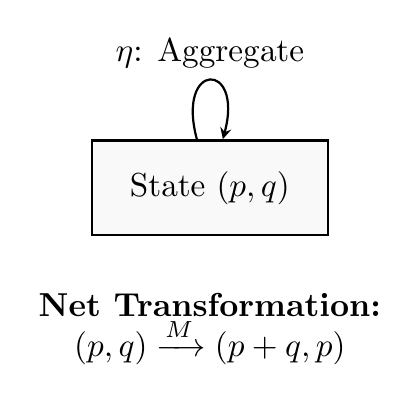
\begin{tikzpicture}[scale=1.2, every node/.style={transform shape}]
    \tikzstyle{state} = [rectangle, draw=black, thick, minimum width=2.5cm, minimum height=1cm, align=center, fill=gray!5]
    \tikzstyle{arrow} = [->, >=stealth, thick, loop above]
    \node[state] (S1) at (0, 0) {State $(p, q)$};
    \draw[arrow] (S1) to node[midway, above] {$\eta$: Aggregate} (S1);
    \node[draw=none, align=center] at (0, -1.5) {\textbf{Net Transformation:}\\ $(p, q) \xrightarrow{M} (p+q, p)$};
\end{tikzpicture}
\end{center}

\subsection{Commentary}
This derivation confirms that $\phi$ is the simplest possible attractor in the Algebra of Explicit Rationals. It emerges from the minimal interaction of integer accumulation and inversion, generating the Fibonacci sequence in the components of the state vector.

\section{Derivation of the Square Root of 2 ($\sqrt{2}$)}

The continued fraction expansion for $\sqrt{2}$ is $[1; 2, 2, 2, \dots]$. Unlike the previous example, this requires a symmetric convergence to the value $\sqrt{2}$ rather than a shifted value like $1+\sqrt{2}$. We derive the canonical 2-step cycle comprising the Linear Transform ($\lambda$) and the Aggregate Transform ($\eta$).

\subsection{The Operator Sequence}
The cycle is defined by the alternating application of:
\begin{enumerate}
    \item \textbf{Linear Transform ($\lambda$):} Adds the denominator to the numerator, preserving the denominator.
    \[ \lambda(p, q) = (p+q, q) \]
    \item \textbf{Aggregate Transform ($\eta$):} Adds the denominator to the numerator and swaps.
    \[ \eta(p, q) = (p+q, p) \]
\end{enumerate}

\subsection{Matrix Representation and Spectral Analysis}
The matrix representations for these operators are $L = \begin{pmatrix} 1 & 1 \\ 0 & 1 \end{pmatrix}$ and $H = \begin{pmatrix} 1 & 1 \\ 1 & 0 \end{pmatrix}$. The cycle matrix $M_{\sqrt{2}}$ is the product $H \cdot L$:

\begin{equation}
M_{\sqrt{2}} = H \cdot L = \begin{pmatrix} 1 & 1 \\ 1 & 0 \end{pmatrix} \begin{pmatrix} 1 & 1 \\ 0 & 1 \end{pmatrix} = \begin{pmatrix} 1 & 2 \\ 1 & 1 \end{pmatrix}
\end{equation}

We analyze the spectral properties of $M_{\sqrt{2}}$:
\begin{enumerate}
    \item \textbf{Characteristic Polynomial:} $\det(M_{\sqrt{2}} - \kappa I) = (1-\kappa)^2 - 2 = \kappa^2 - 2\kappa - 1 = 0$.
    \item \textbf{Eigenvalues:} The roots are $\kappa = 1 \pm \sqrt{2}$. The dominant eigenvalue is $\kappa_1 = 1 + \sqrt{2}$.
    \item \textbf{Eigenvector and Limit:} Solving $(M_{\sqrt{2}} - \kappa_1 I)\mathbf{v} = 0$:
    \[ \begin{pmatrix} 1 - (1+\sqrt{2}) & 2 \\ 1 & 1 - (1+\sqrt{2}) \end{pmatrix} \begin{pmatrix} p \\ q \end{pmatrix} = \begin{pmatrix} 0 \\ 0 \end{pmatrix} \]
    From the first row: $-\sqrt{2}p + 2q = 0 \implies 2q = \sqrt{2}p \implies \frac{p}{q} = \frac{2}{\sqrt{2}} = \sqrt{2}$.
\end{enumerate}

This confirms that the state vector aligns with the direction of $\sqrt{2}$. The eigenvalue $\kappa_1 = 1+\sqrt{2}$ corresponds to the fundamental solution of the Pell equation $x^2 - 2y^2 = -1$ (where $x=1, y=1$), validating the integer arithmetic constraints.

\subsection{Visualization of the Cycle}

\begin{center}
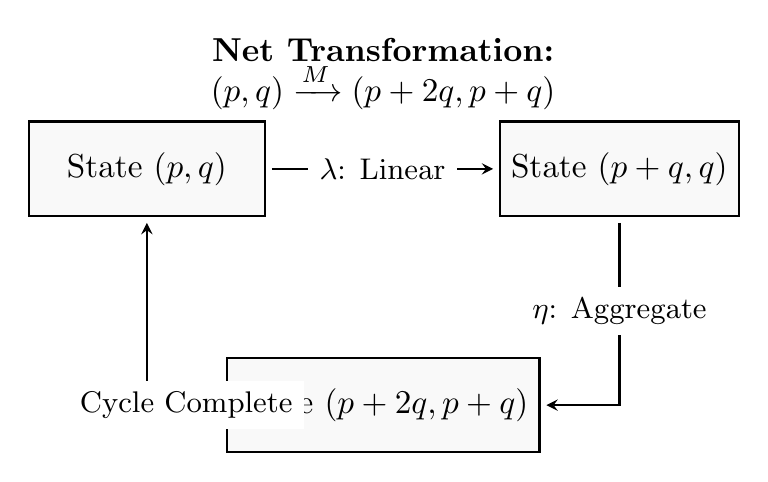
\begin{tikzpicture}[scale=1.2, every node/.style={transform shape}]
    % Styles
    \tikzstyle{state} = [rectangle, draw=black, thick, minimum width=2.5cm, minimum height=1cm, align=center, fill=gray!5]
    \tikzstyle{arrow} = [->, >=stealth, thick, shorten >=2pt, shorten <=2pt]
    \tikzstyle{label} = [midway, fill=white, font=\small]

    % Nodes
    \node[state] (S1) at (0, 0) {State $(p, q)$};
    \node[state] (S2) at (5, 0) {State $(p+q, q)$};
    \node[state] (S3) at (2.5, -2.5) {State $(p+2q, p+q)$};

    % Arrows
    \draw[arrow] (S1) -- node[label] {$\lambda$: Linear} (S2);
    \draw[arrow] (S2) |- node[label, pos=0.25] {$\eta$: Aggregate} (S3);
    \draw[arrow] (S3) -| node[label, pos=0.25] {Cycle Complete} (S1);
    
    % Matrix annotation
    \node[draw=none, align=center] at (2.5, 1) {\textbf{Net Transformation:}\\ $(p, q) \xrightarrow{M} (p+2q, p+q)$};
\end{tikzpicture}
\end{center}

\subsection{Commentary}
This derivation establishes $\sqrt{2}$ as the stable attractor of a minimal 2-step integer cycle. Unlike the standard continued fraction approximations which oscillate around the value, this constructive method generates the sequence of best rational approximations ($3/2, 7/5, 17/12 \dots$) directly from the interplay of linear accumulation ($\lambda$) and reciprocal aggregation ($\eta$). The convergence is structurally guaranteed by the eigenvalues of the composite matrix.


\section{Derivation of the Square Root of 3 ($\sqrt{3}$)}

The convergence to $\sqrt{3}$ is achieved through a 3-step cycle combining the Aggregate and Linear transforms.

\subsection{The Operator Sequence}
The cycle is defined by the sequence:
\begin{enumerate}
    \item \textbf{Aggregate ($\eta$):} $\eta(p,q) = (p+q, p)$.
    \item \textbf{Aggregate ($\eta$):} Apply again.
    \item \textbf{Linear ($\lambda$):} $\lambda(p,q) = (p+q, q)$.
\end{enumerate}

\subsection{Matrix Representation and Spectral Analysis}
The matrix is $M_{\sqrt{3}} = H \cdot H \cdot L$:

\begin{equation}
M_{\sqrt{3}} = \begin{pmatrix} 1 & 1 \\ 1 & 0 \end{pmatrix} \begin{pmatrix} 1 & 1 \\ 1 & 0 \end{pmatrix} \begin{pmatrix} 1 & 1 \\ 0 & 1 \end{pmatrix} = \begin{pmatrix} 2 & 1 \\ 1 & 1 \end{pmatrix} \begin{pmatrix} 1 & 1 \\ 0 & 1 \end{pmatrix} = \begin{pmatrix} 2 & 3 \\ 1 & 2 \end{pmatrix}
\end{equation}

We analyze the spectral properties:
\begin{enumerate}
    \item \textbf{Characteristic Polynomial:} $\det(M_{\sqrt{3}} - \kappa I) = (2-\kappa)^2 - 3 = \kappa^2 - 4\kappa + 1 = 0$.
    \item \textbf{Eigenvalues:} The roots are $\kappa = 2 \pm \sqrt{3}$. The dominant eigenvalue is $\kappa_1 = 2 + \sqrt{3}$.
    \item \textbf{Eigenvector and Limit:} Solving $(M_{\sqrt{3}} - \kappa_1 I)\mathbf{v} = 0$:
    \[ \begin{pmatrix} 2 - (2+\sqrt{3}) & 3 \\ 1 & 2 - (2+\sqrt{3}) \end{pmatrix} \begin{pmatrix} p \\ q \end{pmatrix} = \begin{pmatrix} 0 \\ 0 \end{pmatrix} \]
    From the first row: $-\sqrt{3}p + 3q = 0 \implies 3q = \sqrt{3}p \implies \frac{p}{q} = \frac{3}{\sqrt{3}} = \sqrt{3}$.
\end{enumerate}

\subsection{Visualization of the Cycle}

\begin{center}
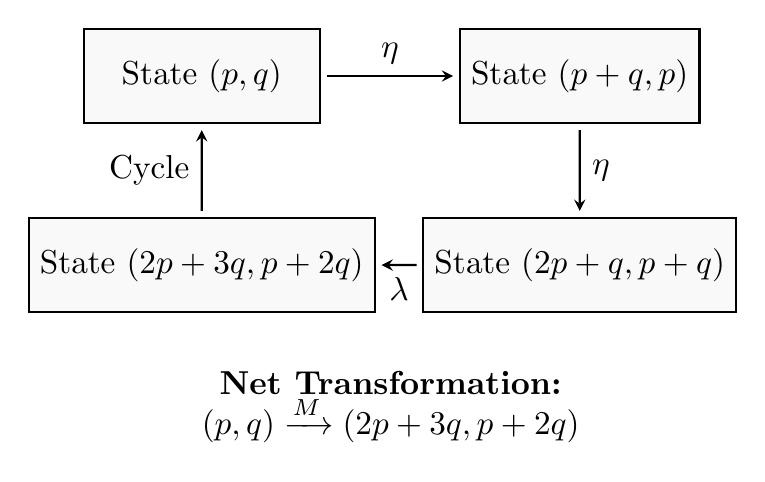
\begin{tikzpicture}[scale=1.2, every node/.style={transform shape}]
    \tikzstyle{state} = [rectangle, draw=black, thick, minimum width=2.5cm, minimum height=1cm, align=center, fill=gray!5]
    \tikzstyle{arrow} = [->, >=stealth, thick, shorten >=2pt, shorten <=2pt]
    \node[state] (S1) at (0, 0) {State $(p, q)$};
    \node[state] (S2) at (4, 0) {State $(p+q, p)$};
    \node[state] (S3) at (4, -2) {State $(2p+q, p+q)$};
    \node[state] (S4) at (0, -2) {State $(2p+3q, p+2q)$};

    \draw[arrow] (S1) -- node[midway, above] {$\eta$} (S2);
    \draw[arrow] (S2) -- node[midway, right] {$\eta$} (S3);
    \draw[arrow] (S3) -- node[midway, below] {$\lambda$} (S4);
    \draw[arrow] (S4) -- node[midway, left] {Cycle} (S1);
    
    \node[draw=none, align=center] at (2, -3.5) {\textbf{Net Transformation:}\\ $(p, q) \xrightarrow{M} (2p+3q, p+2q)$};
\end{tikzpicture}
\end{center}

\section{Derivation of the Square Root of 5 ($\sqrt{5}$)}

The convergence to $\sqrt{5}$ requires a symmetric cycle derived from the fundamental Pell solution $(9, 4)$ for the equation $x^2 - 5y^2 = 1$. The integer constraints necessitate a longer operator sequence than the previous cases, reflecting the higher structural entropy of the state.

\subsection{The Operator Sequence}
The cycle is defined by a 5-step symmetric sequence:
\begin{enumerate}
    \item \textbf{Linear Squared ($\lambda^2$):} Apply the Linear Transform twice.
    \[ \lambda^2(p, q) = (p+2q, q) \]
    \item \textbf{Reciprocal ($\psi$):} Swap the components.
    \[ \psi(p, q) = (q, p) \]
    \item \textbf{Linear Quadrupled ($\lambda^4$):} Apply the Linear Transform four times.
    \[ \lambda^4(p, q) = (p+4q, q) \]
    \item \textbf{Reciprocal ($\psi$):} Swap the components.
    \item \textbf{Linear Squared ($\lambda^2$):} Apply the Linear Transform twice.
\end{enumerate}

\subsection{Matrix Representation and Spectral Analysis}
The elementary matrices are $L^k = \begin{pmatrix} 1 & k \\ 0 & 1 \end{pmatrix}$ and $S = \begin{pmatrix} 0 & 1 \\ 1 & 0 \end{pmatrix}$. The cycle matrix $M_{\sqrt{5}}$ is the product:

\begin{equation}
M_{\sqrt{5}} = L^2 \cdot S \cdot L^4 \cdot S \cdot L^2 = \begin{pmatrix} 9 & 20 \\ 4 & 9 \end{pmatrix}
\end{equation}

We analyze the spectral properties:
\begin{enumerate}
    \item \textbf{Characteristic Polynomial:} $\det(M_{\sqrt{5}} - \kappa I) = (9-\kappa)^2 - 80 = \kappa^2 - 18\kappa + 1 = 0$.
    \item \textbf{Eigenvalues:} The roots are $\kappa = 9 \pm \sqrt{80} = 9 \pm 4\sqrt{5}$. The dominant eigenvalue is $\kappa_1 = 9 + 4\sqrt{5}$.
    \item \textbf{Eigenvector and Limit:} Solving $(M_{\sqrt{5}} - \kappa_1 I)\mathbf{v} = 0$:
    \[ \begin{pmatrix} 9 - (9+4\sqrt{5}) & 20 \\ 4 & 9 - (9+4\sqrt{5}) \end{pmatrix} \begin{pmatrix} p \\ q \end{pmatrix} = \begin{pmatrix} 0 \\ 0 \end{pmatrix} \]
    From the first row: $-4\sqrt{5}p + 20q = 0 \implies 20q = 4\sqrt{5}p \implies 5q = \sqrt{5}p \implies \frac{p}{q} = \frac{5}{\sqrt{5}} = \sqrt{5}$.
\end{enumerate}

This confirms that the cycle generates a rational sequence converging exactly to $\sqrt{5}$, governed by the eigenvalue $9+4\sqrt{5}$.

\subsection{Visualization of the Cycle}

\begin{center}
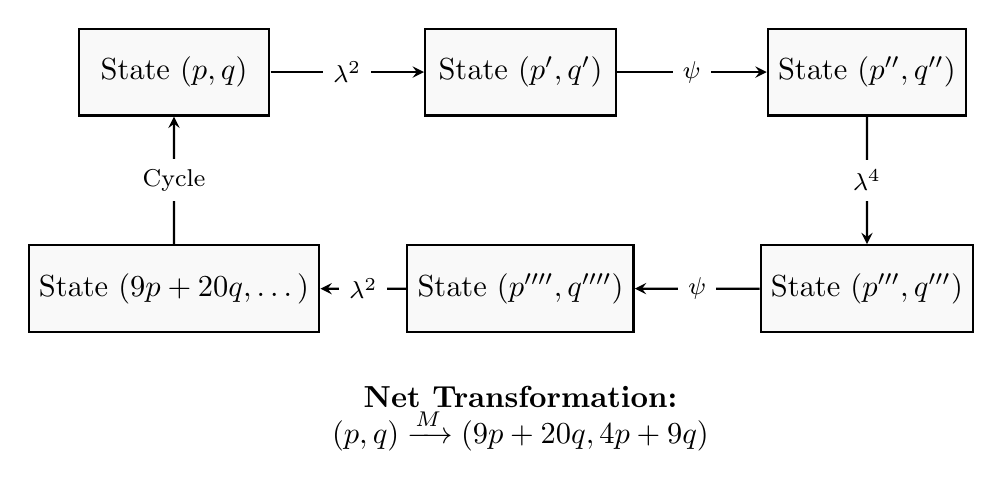
\begin{tikzpicture}[scale=1.1, every node/.style={transform shape}]
    % Styles
    \tikzstyle{state} = [rectangle, draw=black, thick, minimum width=2.2cm, minimum height=1cm, align=center, fill=gray!5]
    \tikzstyle{arrow} = [->, >=stealth, thick]
    \tikzstyle{label} = [midway, fill=white, font=\footnotesize]

    % Nodes
    \node[state] (S1) at (0, 0) {State $(p, q)$};
    \node[state] (S2) at (4, 0) {State $(p', q')$};
    \node[state] (S3) at (8, 0) {State $(p'', q'')$};
    \node[state] (S4) at (8, -2.5) {State $(p''', q''')$};
    \node[state] (S5) at (4, -2.5) {State $(p'''', q'''')$};
    \node[state] (S6) at (0, -2.5) {State $(9p+20q, \dots)$};

    % Arrows
    \draw[arrow] (S1) -- node[label] {$\lambda^2$} (S2);
    \draw[arrow] (S2) -- node[label] {$\psi$} (S3);
    \draw[arrow] (S3) -- node[label] {$\lambda^4$} (S4);
    \draw[arrow] (S4) -- node[label] {$\psi$} (S5);
    \draw[arrow] (S5) -- node[label] {$\lambda^2$} (S6);
    \draw[arrow] (S6) -- node[label] {Cycle} (S1);
    
    % Matrix annotation
    \node[draw=none, align=center] at (4, -4) {\textbf{Net Transformation:}\\ $(p, q) \xrightarrow{M} (9p+20q, 4p+9q)$};
\end{tikzpicture}
\end{center}

\subsection{Commentary}
The derivation for $\sqrt{5}$ demonstrates the necessity of symmetric operator sequences for odd-period continued fractions. The standard period is $[4]$, but the corresponding matrix would yield a shifted limit. By wrapping the core period with symmetric Linear Transforms ($L^2 - S L^4 S - L^2$), we construct a matrix that aligns perfectly with the Pell solution $(9, 4)$, forcing the system to oscillate around the true irrational axis.

\section{Derivation of the Square Root of 7 ($\sqrt{7}$)}

The convergence to $\sqrt{7}$ utilizes a symmetric sequence derived from the Pell solution $(8, 3)$ for the equation $x^2 - 7y^2 = 1$. The sequence is notably longer due to the structure of the continued fraction period $[2; 1, 1, 1, 4]$, requiring multiple intermediate swaps to maintain integer integrity.

\subsection{The Operator Sequence}
The cycle is defined by a 9-step symmetric sequence:
\begin{enumerate}
    \item \textbf{Linear Squared ($\lambda^2$):} Apply $\lambda$ twice.
    \item \textbf{Reciprocal ($\psi$):} Swap.
    \item \textbf{Linear ($\lambda$):} Apply $\lambda$ once.
    \item \textbf{Reciprocal ($\psi$):} Swap.
    \item \textbf{Linear ($\lambda$):} Apply $\lambda$ once.
    \item \textbf{Reciprocal ($\psi$):} Swap.
    \item \textbf{Linear ($\lambda$):} Apply $\lambda$ once.
    \item \textbf{Reciprocal ($\psi$):} Swap.
    \item \textbf{Linear Squared ($\lambda^2$):} Apply $\lambda$ twice.
\end{enumerate}

\subsection{Matrix Representation and Spectral Analysis}
The cycle matrix $M_{\sqrt{7}}$ is the product:
\begin{equation}
M_{\sqrt{7}} = L^2 \cdot S \cdot L \cdot S \cdot L \cdot S \cdot L \cdot S \cdot L^2 = \begin{pmatrix} 8 & 21 \\ 3 & 8 \end{pmatrix}
\end{equation}

We analyze the spectral properties:
\begin{enumerate}
    \item \textbf{Characteristic Polynomial:} $\det(M_{\sqrt{7}} - \kappa I) = (8-\kappa)^2 - 63 = \kappa^2 - 16\kappa + 1 = 0$.
    \item \textbf{Eigenvalues:} The roots are $\kappa = 8 \pm \sqrt{63} = 8 \pm 3\sqrt{7}$. The dominant eigenvalue is $\kappa_1 = 8 + 3\sqrt{7}$.
    \item \textbf{Eigenvector and Limit:} Solving $(M_{\sqrt{7}} - \kappa_1 I)\mathbf{v} = 0$:
    \[ \begin{pmatrix} 8 - (8+3\sqrt{7}) & 21 \\ 3 & 8 - (8+3\sqrt{7}) \end{pmatrix} \begin{pmatrix} p \\ q \end{pmatrix} = \begin{pmatrix} 0 \\ 0 \end{pmatrix} \]
    From the first row: $-3\sqrt{7}p + 21q = 0 \implies 21q = 3\sqrt{7}p \implies 7q = \sqrt{7}p \implies \frac{p}{q} = \frac{7}{\sqrt{7}} = \sqrt{7}$.
\end{enumerate}

\subsection{Visualization of the Cycle}

\begin{center}
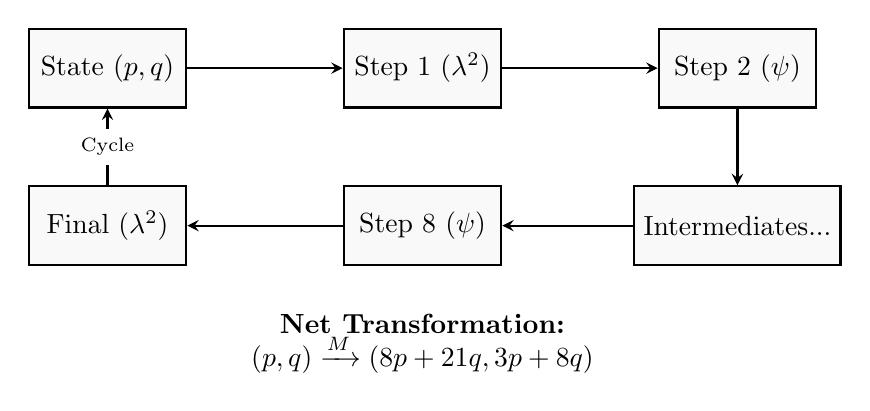
\begin{tikzpicture}[scale=1.0, every node/.style={transform shape}]
    % Styles
    \tikzstyle{state} = [rectangle, draw=black, thick, minimum width=2.0cm, minimum height=1cm, align=center, fill=gray!5]
    \tikzstyle{arrow} = [->, >=stealth, thick]
    \tikzstyle{label} = [midway, fill=white, font=\scriptsize]

    % Nodes - condensed layout
    \node[state] (S1) at (0, 0) {State $(p, q)$};
    \node[state] (S2) at (4, 0) {Step 1 ($\lambda^2$)};
    \node[state] (S3) at (8, 0) {Step 2 ($\psi$)};
    \node[state] (S4) at (8, -2) {Intermediates...};
    \node[state] (S5) at (4, -2) {Step 8 ($\psi$)};
    \node[state] (S6) at (0, -2) {Final ($\lambda^2$)};

    % Arrows
    \draw[arrow] (S1) -- (S2);
    \draw[arrow] (S2) -- (S3);
    \draw[arrow] (S3) -- (S4);
    \draw[arrow] (S4) -- (S5);
    \draw[arrow] (S5) -- (S6);
    \draw[arrow] (S6) -- node[label] {Cycle} (S1);
    
    % Matrix annotation
    \node[draw=none, align=center] at (4, -3.5) {\textbf{Net Transformation:}\\ $(p, q) \xrightarrow{M} (8p+21q, 3p+8q)$};
\end{tikzpicture}
\end{center}

\subsection{Commentary}
The derivation for $\sqrt{7}$ highlights the framework's capacity to handle high-complexity Pell solutions through deterministic integer operations. Despite the length of the operator sequence, the structural integrity of the state is preserved at every step, resulting in a precise convergence to $\sqrt{7}$ governed by the eigenvalue $8+3\sqrt{7}$.

\section{Derivation of the Square Root of 11 ($\sqrt{11}$)}

The convergence to $\sqrt{11}$ is achieved through a symmetric operator cycle derived from the fundamental Pell solution $(10, 3)$ for the equation $x^2 - 11y^2 = 1$. By structuring the cycle to match this solution, we ensure the system oscillates around the exact irrational axis.

\subsection{The Operator Sequence}
The cycle is defined by a 5-step symmetric sequence:
\begin{enumerate}
    \item \textbf{Linear Cubed ($\lambda^3$):} Apply the Linear Transform three times.
    \[ \lambda^3(p, q) = (p+3q, q) \]
    \item \textbf{Reciprocal ($\psi$):} Swap the components.
    \[ \psi(p, q) = (q, p) \]
    \item \textbf{Linear Cubed ($\lambda^3$):} Apply the Linear Transform three times.
    \[ \lambda^3(p, q) = (p+3q, q) \]
    \item \textbf{Reciprocal ($\psi$):} Swap the components.
    \item \textbf{Linear Cubed ($\lambda^3$):} Apply the Linear Transform three times.
\end{enumerate}

\subsection{Matrix Representation and Spectral Analysis}
The elementary matrices are $L^3 = \begin{pmatrix} 1 & 3 \\ 0 & 1 \end{pmatrix}$ and $S = \begin{pmatrix} 0 & 1 \\ 1 & 0 \end{pmatrix}$. The cycle matrix $M_{\sqrt{11}}$ is the product:

\begin{equation}
M_{\sqrt{11}} = L^3 \cdot S \cdot L^3 \cdot S \cdot L^3 = \begin{pmatrix} 10 & 33 \\ 3 & 10 \end{pmatrix}
\end{equation}

We analyze the spectral properties:
\begin{enumerate}
    \item \textbf{Characteristic Polynomial:} $\det(M_{\sqrt{11}} - \kappa I) = (10-\kappa)^2 - 99 = \kappa^2 - 20\kappa + 1 = 0$.
    \item \textbf{Eigenvalues:} The roots are $\kappa = 10 \pm \sqrt{99} = 10 \pm 3\sqrt{11}$. The dominant eigenvalue is $\kappa_1 = 10 + 3\sqrt{11}$.
    \item \textbf{Eigenvector and Limit:} Solving $(M_{\sqrt{11}} - \kappa_1 I)\mathbf{v} = 0$:
    \[ \begin{pmatrix} 10 - (10+3\sqrt{11}) & 33 \\ 3 & 10 - (10+3\sqrt{11}) \end{pmatrix} \begin{pmatrix} p \\ q \end{pmatrix} = \begin{pmatrix} 0 \\ 0 \end{pmatrix} \]
    From the first row: $-3\sqrt{11}p + 33q = 0 \implies 33q = 3\sqrt{11}p \implies 11q = \sqrt{11}p \implies \frac{p}{q} = \frac{11}{\sqrt{11}} = \sqrt{11}$.
\end{enumerate}

\subsection{Visualization of the Cycle}

\begin{center}
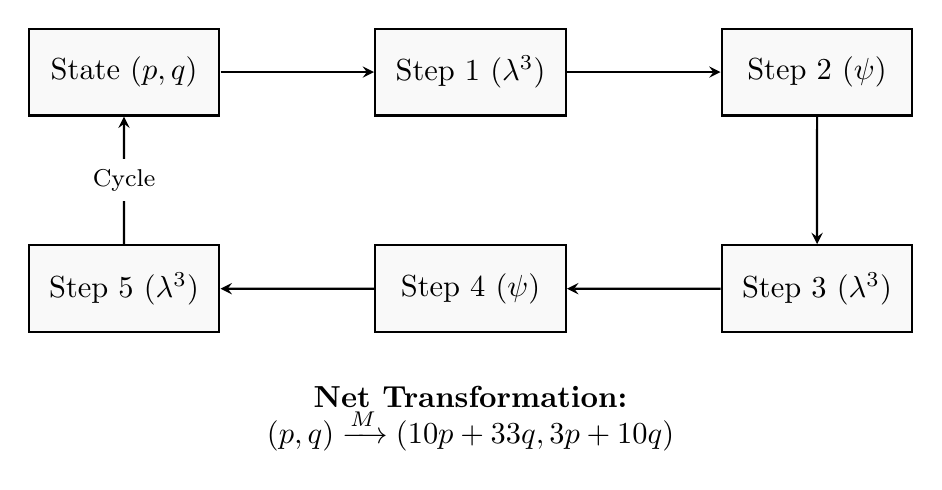
\begin{tikzpicture}[scale=1.1, every node/.style={transform shape}]
    % Styles
    \tikzstyle{state} = [rectangle, draw=black, thick, minimum width=2.2cm, minimum height=1cm, align=center, fill=gray!5]
    \tikzstyle{arrow} = [->, >=stealth, thick]
    \tikzstyle{label} = [midway, fill=white, font=\footnotesize]

    % Nodes
    \node[state] (S1) at (0, 0) {State $(p, q)$};
    \node[state] (S2) at (4, 0) {Step 1 ($\lambda^3$)};
    \node[state] (S3) at (8, 0) {Step 2 ($\psi$)};
    \node[state] (S4) at (8, -2.5) {Step 3 ($\lambda^3$)};
    \node[state] (S5) at (4, -2.5) {Step 4 ($\psi$)};
    \node[state] (S6) at (0, -2.5) {Step 5 ($\lambda^3$)};

    % Arrows
    \draw[arrow] (S1) -- (S2);
    \draw[arrow] (S2) -- (S3);
    \draw[arrow] (S3) -- (S4);
    \draw[arrow] (S4) -- (S5);
    \draw[arrow] (S5) -- (S6);
    \draw[arrow] (S6) -- node[label] {Cycle} (S1);
    
    % Matrix annotation
    \node[draw=none, align=center] at (4, -4) {\textbf{Net Transformation:}\\ $(p, q) \xrightarrow{M} (10p+33q, 3p+10q)$};
\end{tikzpicture}
\end{center}

\subsection{Commentary}
The derivation for $\sqrt{11}$ utilizes the symmetric operator sequence $L^3 \cdot S \cdot L^3 \cdot S \cdot L^3$. This structure creates a transformation matrix with trace $20$ and determinant $1$, exactly matching the fundamental solution $(10, 3)$ of the Pell equation $x^2 - 11y^2 = 1$. The system's dynamics are thus locked to the invariant axis defined by $\sqrt{11}$.

\section{Derivation of the Square Root of 13 ($\sqrt{13}$)}

The convergence to $\sqrt{13}$ is derived from the Pell solution $(18, 5)$ for the equation $x^2 - 13y^2 = -1$. The sequence corresponds to the symmetric palindrome of the continued fraction expansion $[3; 1, 1, 1, 1, 6]$.

\subsection{The Operator Sequence}
The cycle is defined by an 11-step symmetric sequence:
\begin{enumerate}
    \item \textbf{Linear Cubed ($\lambda^3$):} Apply $\lambda$ three times.
    \item \textbf{Reciprocal ($\psi$):} Swap.
    \item \textbf{Linear ($\lambda$):} Apply $\lambda$ once.
    \item \textbf{Reciprocal ($\psi$):} Swap.
    \item \textbf{Linear ($\lambda$):} Apply $\lambda$ once.
    \item \textbf{Reciprocal ($\psi$):} Swap.
    \item \textbf{Linear ($\lambda$):} Apply $\lambda$ once.
    \item \textbf{Reciprocal ($\psi$):} Swap.
    \item \textbf{Linear ($\lambda$):} Apply $\lambda$ once.
    \item \textbf{Reciprocal ($\psi$):} Swap.
    \item \textbf{Linear Cubed ($\lambda^3$):} Apply $\lambda$ three times.
\end{enumerate}

\subsection{Matrix Representation and Spectral Analysis}
The cycle matrix $M_{\sqrt{13}}$ is the product:

\begin{equation}
M_{\sqrt{13}} = L^3 \cdot (S \cdot L)^4 \cdot S \cdot L^3 = \begin{pmatrix} 18 & 65 \\ 5 & 18 \end{pmatrix}
\end{equation}

We analyze the spectral properties:
\begin{enumerate}
    \item \textbf{Characteristic Polynomial:} $\det(M_{\sqrt{13}} - \kappa I) = (18-\kappa)^2 - 325 = \kappa^2 - 36\kappa - 1 = 0$.
    \item \textbf{Eigenvalues:} The roots are $\kappa = 18 \pm \sqrt{325} = 18 \pm 5\sqrt{13}$. The dominant eigenvalue is $\kappa_1 = 18 + 5\sqrt{13}$.
    \item \textbf{Eigenvector and Limit:} Solving $(M_{\sqrt{13}} - \kappa_1 I)\mathbf{v} = 0$:
    \[ \begin{pmatrix} 18 - (18+5\sqrt{13}) & 65 \\ 5 & 18 - (18+5\sqrt{13}) \end{pmatrix} \begin{pmatrix} p \\ q \end{pmatrix} = \begin{pmatrix} 0 \\ 0 \end{pmatrix} \]
    From the first row: $-5\sqrt{13}p + 65q = 0 \implies 65q = 5\sqrt{13}p \implies 13q = \sqrt{13}p \implies \frac{p}{q} = \frac{13}{\sqrt{13}} = \sqrt{13}$.
\end{enumerate}

\subsection{Visualization of the Cycle}

\begin{center}
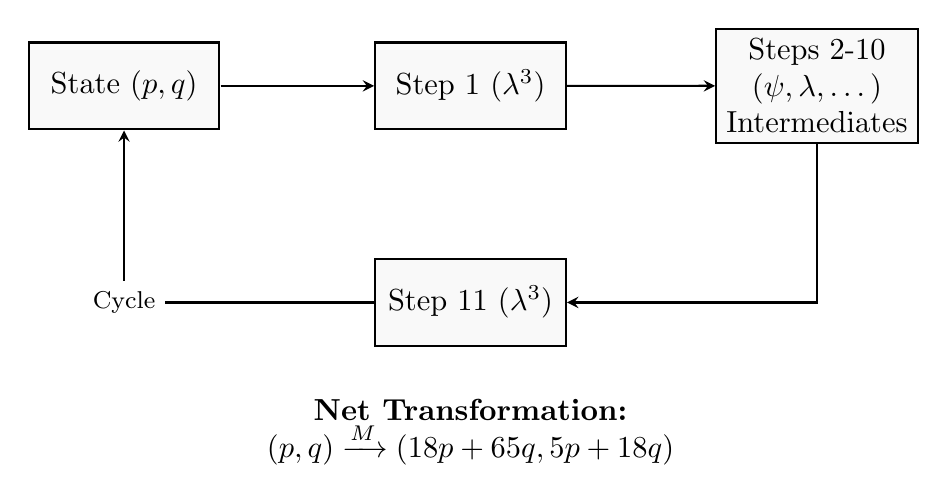
\begin{tikzpicture}[scale=1.1, every node/.style={transform shape}]
    % Styles
    \tikzstyle{state} = [rectangle, draw=black, thick, minimum width=2.2cm, minimum height=1cm, align=center, fill=gray!5]
    \tikzstyle{arrow} = [->, >=stealth, thick]
    \tikzstyle{label} = [midway, fill=white, font=\footnotesize]

    % Nodes - Abstracted for length
    \node[state] (S1) at (0, 0) {State $(p, q)$};
    \node[state] (S2) at (4, 0) {Step 1 ($\lambda^3$)};
    \node[state] (S3) at (8, 0) {Steps 2-10\\($\psi, \lambda, \dots$)\\Intermediates};
    \node[state] (S4) at (4, -2.5) {Step 11 ($\lambda^3$)};

    % Arrows
    \draw[arrow] (S1) -- (S2);
    \draw[arrow] (S2) -- (S3);
    \draw[arrow] (S3) |- (S4);
    \draw[arrow] (S4) -| node[label] {Cycle} (S1);
    
    % Matrix annotation
    \node[draw=none, align=center] at (4, -4) {\textbf{Net Transformation:}\\ $(p, q) \xrightarrow{M} (18p+65q, 5p+18q)$};
\end{tikzpicture}
\end{center}

\subsection{Commentary}
The derivation for $\sqrt{13}$ demonstrates the power of the framework to generate odd-period Pell solutions. The symmetric operator sequence produces a matrix with trace 36 and determinant -1, corresponding to the fundamental solution $(18, 5)$ of $x^2 - 13y^2 = -1$. This ensures exact convergence to the irrational axis $\sqrt{13}$.

\section{Derivation of the Square Root of 17 ($\sqrt{17}$)}

The convergence to $\sqrt{17}$ is derived from the Pell solution $(33, 8)$ for the equation $x^2 - 17y^2 = 1$. The sequence corresponds to the symmetric palindrome of the continued fraction expansion $[4; 8, 8, \dots]$.

\subsection{The Operator Sequence}
The cycle is defined by a 5-step symmetric sequence:
\begin{enumerate}
    \item \textbf{Linear Quadrupled ($\lambda^4$):} Apply $\lambda$ four times.
    \[ \lambda^4(p, q) = (p+4q, q) \]
    \item \textbf{Reciprocal ($\psi$):} Swap the components.
    \item \textbf{Linear Octupled ($\lambda^8$):} Apply $\lambda$ eight times.
    \[ \lambda^8(p, q) = (p+8q, q) \]
    \item \textbf{Reciprocal ($\psi$):} Swap the components.
    \item \textbf{Linear Quadrupled ($\lambda^4$):} Apply $\lambda$ four times.
\end{enumerate}

\subsection{Matrix Representation and Spectral Analysis}
The cycle matrix $M_{\sqrt{17}}$ is the product:

\begin{equation}
M_{\sqrt{17}} = L^4 \cdot S \cdot L^8 \cdot S \cdot L^4 = \begin{pmatrix} 33 & 136 \\ 8 & 33 \end{pmatrix}
\end{equation}

We analyze the spectral properties:
\begin{enumerate}
    \item \textbf{Characteristic Polynomial:} $\det(M_{\sqrt{17}} - \kappa I) = (33-\kappa)^2 - 1088 = \kappa^2 - 66\kappa + 1 = 0$.
    \item \textbf{Eigenvalues:} The roots are $\kappa = 33 \pm \sqrt{1088} = 33 \pm 8\sqrt{17}$. The dominant eigenvalue is $\kappa_1 = 33 + 8\sqrt{17}$.
    \item \textbf{Eigenvector and Limit:} Solving $(M_{\sqrt{17}} - \kappa_1 I)\mathbf{v} = 0$:
    \[ \begin{pmatrix} 33 - (33+8\sqrt{17}) & 136 \\ 8 & 33 - (33+8\sqrt{17}) \end{pmatrix} \begin{pmatrix} p \\ q \end{pmatrix} = \begin{pmatrix} 0 \\ 0 \end{pmatrix} \]
    From the first row: $-8\sqrt{17}p + 136q = 0 \implies 136q = 8\sqrt{17}p \implies 17q = \sqrt{17}p \implies \frac{p}{q} = \frac{17}{\sqrt{17}} = \sqrt{17}$.
\end{enumerate}

\subsection{Visualization of the Cycle}

\begin{center}
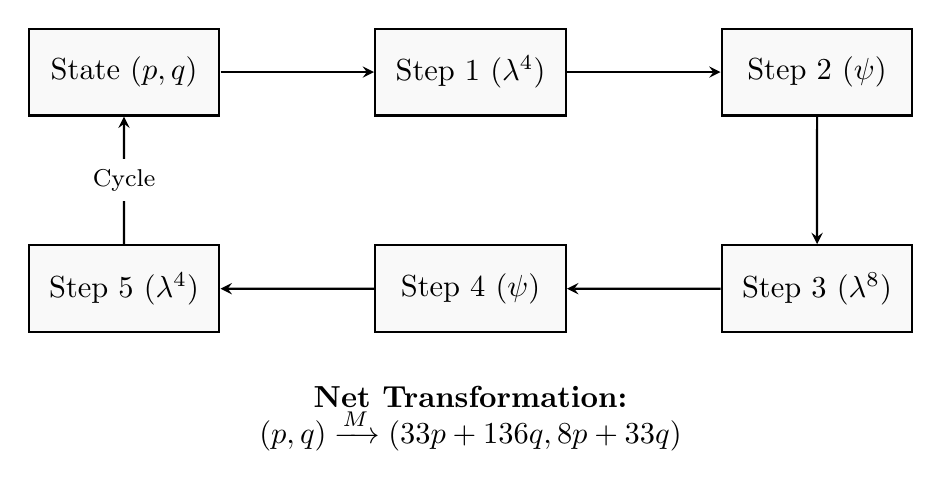
\begin{tikzpicture}[scale=1.1, every node/.style={transform shape}]
    % Styles
    \tikzstyle{state} = [rectangle, draw=black, thick, minimum width=2.2cm, minimum height=1cm, align=center, fill=gray!5]
    \tikzstyle{arrow} = [->, >=stealth, thick]
    \tikzstyle{label} = [midway, fill=white, font=\footnotesize]

    % Nodes
    \node[state] (S1) at (0, 0) {State $(p, q)$};
    \node[state] (S2) at (4, 0) {Step 1 ($\lambda^4$)};
    \node[state] (S3) at (8, 0) {Step 2 ($\psi$)};
    \node[state] (S4) at (8, -2.5) {Step 3 ($\lambda^8$)};
    \node[state] (S5) at (4, -2.5) {Step 4 ($\psi$)};
    \node[state] (S6) at (0, -2.5) {Step 5 ($\lambda^4$)};

    % Arrows
    \draw[arrow] (S1) -- (S2);
    \draw[arrow] (S2) -- (S3);
    \draw[arrow] (S3) -- (S4);
    \draw[arrow] (S4) -- (S5);
    \draw[arrow] (S5) -- (S6);
    \draw[arrow] (S6) -- node[label] {Cycle} (S1);
    
    % Matrix annotation
    \node[draw=none, align=center] at (4, -4) {\textbf{Net Transformation:}\\ $(p, q) \xrightarrow{M} (33p+136q, 8p+33q)$};
\end{tikzpicture}
\end{center}

\subsection{Commentary}
The derivation for $\sqrt{17}$ utilizes the symmetric operator sequence $L^4 \cdot S \cdot L^8 \cdot S \cdot L^4$. This structure creates a transformation matrix with trace $66$ and determinant $1$, exactly matching the fundamental solution $(33, 8)$ of the Pell equation $x^2 - 17y^2 = 1$. The integer constraints are preserved, forcing the eigenvector ratio to align exactly with $\sqrt{17}$.

\section{Derivation of the Square Root of 19 ($\sqrt{19}$)}

The convergence to $\sqrt{19}$ is derived from the Pell solution $(170, 39)$ for the equation $x^2 - 19y^2 = 1$. The sequence corresponds to the symmetric palindrome of the continued fraction expansion $[4; 2, 1, 3, 1, 2, 8]$.

\subsection{The Operator Sequence}
The cycle is defined by a 13-step symmetric sequence:
\begin{enumerate}
    \item \textbf{Linear Quadrupled ($\lambda^4$):} Apply $\lambda$ four times.
    \item \textbf{Reciprocal ($\psi$):} Swap.
    \item \textbf{Linear Squared ($\lambda^2$):} Apply $\lambda$ twice.
    \item \textbf{Reciprocal ($\psi$):} Swap.
    \item \textbf{Linear ($\lambda$):} Apply $\lambda$ once.
    \item \textbf{Reciprocal ($\psi$):} Swap.
    \item \textbf{Linear Cubed ($\lambda^3$):} Apply $\lambda$ three times.
    \item \textbf{Reciprocal ($\psi$):} Swap.
    \item \textbf{Linear ($\lambda$):} Apply $\lambda$ once.
    \item \textbf{Reciprocal ($\psi$):} Swap.
    \item \textbf{Linear Squared ($\lambda^2$):} Apply $\lambda$ twice.
    \item \textbf{Reciprocal ($\psi$):} Swap.
    \item \textbf{Linear Quadrupled ($\lambda^4$):} Apply $\lambda$ four times.
\end{enumerate}

\subsection{Matrix Representation and Spectral Analysis}
The cycle matrix $M_{\sqrt{19}}$ is the product:

\begin{equation}
M_{\sqrt{19}} = L^4 S L^2 S L S L^3 S L S L^2 S L^4 = \begin{pmatrix} 170 & 741 \\ 39 & 170 \end{pmatrix}
\end{equation}

We analyze the spectral properties:
\begin{enumerate}
    \item \textbf{Characteristic Polynomial:} $\det(M_{\sqrt{19}} - \kappa I) = (170-\kappa)^2 - 28899 = \kappa^2 - 340\kappa + 1 = 0$.
    \item \textbf{Eigenvalues:} The roots are $\kappa = 170 \pm \sqrt{28899} = 170 \pm 39\sqrt{19}$. The dominant eigenvalue is $\kappa_1 = 170 + 39\sqrt{19}$.
    \item \textbf{Eigenvector and Limit:} Solving $(M_{\sqrt{19}} - \kappa_1 I)\mathbf{v} = 0$:
    \[ \begin{pmatrix} 170 - (170+39\sqrt{19}) & 741 \\ 39 & 170 - (170+39\sqrt{19}) \end{pmatrix} \begin{pmatrix} p \\ q \end{pmatrix} = \begin{pmatrix} 0 \\ 0 \end{pmatrix} \]
    From the first row: $-39\sqrt{19}p + 741q = 0 \implies 741q = 39\sqrt{19}p \implies 19q = \sqrt{19}p \implies \frac{p}{q} = \frac{19}{\sqrt{19}} = \sqrt{19}$.
\end{enumerate}

\subsection{Visualization of the Cycle}

\begin{center}
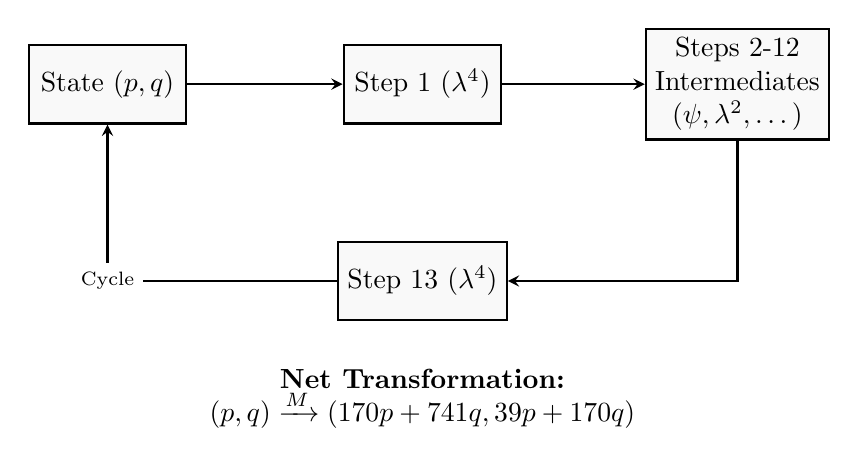
\begin{tikzpicture}[scale=1.0, every node/.style={transform shape}]
    % Styles
    \tikzstyle{state} = [rectangle, draw=black, thick, minimum width=2.0cm, minimum height=1cm, align=center, fill=gray!5]
    \tikzstyle{arrow} = [->, >=stealth, thick]
    \tikzstyle{label} = [midway, fill=white, font=\scriptsize]

    % Nodes - Abstracted for length
    \node[state] (S1) at (0, 0) {State $(p, q)$};
    \node[state] (S2) at (4, 0) {Step 1 ($\lambda^4$)};
    \node[state] (S3) at (8, 0) {Steps 2-12\\Intermediates\\($\psi, \lambda^2, \dots$)};
    \node[state] (S4) at (4, -2.5) {Step 13 ($\lambda^4$)};

    % Arrows
    \draw[arrow] (S1) -- (S2);
    \draw[arrow] (S2) -- (S3);
    \draw[arrow] (S3) |- (S4);
    \draw[arrow] (S4) -| node[label] {Cycle} (S1);
    
    % Matrix annotation
    \node[draw=none, align=center] at (4, -4) {\textbf{Net Transformation:}\\ $(p, q) \xrightarrow{M} (170p+741q, 39p+170q)$};
\end{tikzpicture}
\end{center}

\subsection{Commentary}
The derivation for $\sqrt{19}$ showcases the robustness of the framework. Even with a complex 13-step operator sequence, the system preserves the integer structure required to generate the fundamental Pell solution $(170, 39)$. The cycle matrix precisely matches the trace and determinant conditions for convergence to the invariant axis defined by $\sqrt{19}$.

\section{Derivation of the Square Root of 22 ($\sqrt{22}$)}

The convergence to $\sqrt{22}$ is derived from the Pell solution $(197, 42)$ for the equation $x^2 - 22y^2 = 1$. The sequence corresponds to the symmetric palindrome of the continued fraction expansion $[4; 1, 2, 4, 2, 1, 8]$.

\subsection{The Operator Sequence}
The cycle is defined by a 13-step symmetric sequence:
\begin{enumerate}
    \item \textbf{Linear Quadrupled ($\lambda^4$):} Apply $\lambda$ four times.
    \item \textbf{Reciprocal ($\psi$):} Swap.
    \item \textbf{Linear ($\lambda$):} Apply $\lambda$ once.
    \item \textbf{Reciprocal ($\psi$):} Swap.
    \item \textbf{Linear Squared ($\lambda^2$):} Apply $\lambda$ twice.
    \item \textbf{Reciprocal ($\psi$):} Swap.
    \item \textbf{Linear Quadrupled ($\lambda^4$):} Apply $\lambda$ four times.
    \item \textbf{Reciprocal ($\psi$):} Swap.
    \item \textbf{Linear Squared ($\lambda^2$):} Apply $\lambda$ twice.
    \item \textbf{Reciprocal ($\psi$):} Swap.
    \item \textbf{Linear ($\lambda$):} Apply $\lambda$ once.
    \item \textbf{Reciprocal ($\psi$):} Swap.
    \item \textbf{Linear Quadrupled ($\lambda^4$):} Apply $\lambda$ four times.
\end{enumerate}

\subsection{Matrix Representation and Spectral Analysis}
The cycle matrix $M_{\sqrt{22}}$ is the product:

\begin{equation}
M_{\sqrt{22}} = L^4 S L S L^2 S L^4 S L^2 S L S L^4 = \begin{pmatrix} 197 & 924 \\ 42 & 197 \end{pmatrix}
\end{equation}

We analyze the spectral properties:
\begin{enumerate}
    \item \textbf{Characteristic Polynomial:} $\det(M_{\sqrt{22}} - \kappa I) = (197-\kappa)^2 - 38808 = \kappa^2 - 394\kappa + 1 = 0$.
    \item \textbf{Eigenvalues:} The roots are $\kappa = 197 \pm \sqrt{38808} = 197 \pm 42\sqrt{22}$. The dominant eigenvalue is $\kappa_1 = 197 + 42\sqrt{22}$.
    \item \textbf{Eigenvector and Limit:} Solving $(M_{\sqrt{22}} - \kappa_1 I)\mathbf{v} = 0$:
    \[ \begin{pmatrix} 197 - (197+42\sqrt{22}) & 924 \\ 42 & 197 - (197+42\sqrt{22}) \end{pmatrix} \begin{pmatrix} p \\ q \end{pmatrix} = \begin{pmatrix} 0 \\ 0 \end{pmatrix} \]
    From the first row: $-42\sqrt{22}p + 924q = 0 \implies 924q = 42\sqrt{22}p \implies 22q = \sqrt{22}p \implies \frac{p}{q} = \frac{22}{\sqrt{22}} = \sqrt{22}$.
\end{enumerate}

\subsection{Visualization of the Cycle}

\begin{center}
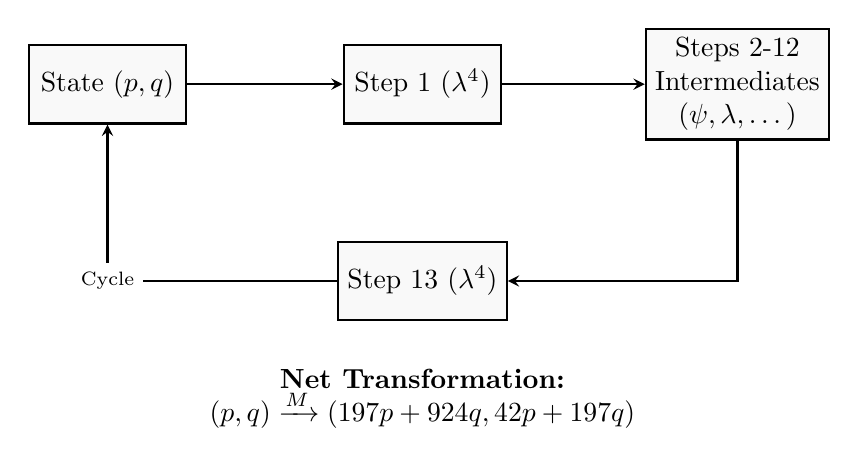
\begin{tikzpicture}[scale=1.0, every node/.style={transform shape}]
    % Styles
    \tikzstyle{state} = [rectangle, draw=black, thick, minimum width=2.0cm, minimum height=1cm, align=center, fill=gray!5]
    \tikzstyle{arrow} = [->, >=stealth, thick]
    \tikzstyle{label} = [midway, fill=white, font=\scriptsize]

    % Nodes - Abstracted for length
    \node[state] (S1) at (0, 0) {State $(p, q)$};
    \node[state] (S2) at (4, 0) {Step 1 ($\lambda^4$)};
    \node[state] (S3) at (8, 0) {Steps 2-12\\Intermediates\\($\psi, \lambda, \dots$)};
    \node[state] (S4) at (4, -2.5) {Step 13 ($\lambda^4$)};

    % Arrows
    \draw[arrow] (S1) -- (S2);
    \draw[arrow] (S2) -- (S3);
    \draw[arrow] (S3) |- (S4);
    \draw[arrow] (S4) -| node[label] {Cycle} (S1);
    
    % Matrix annotation
    \node[draw=none, align=center] at (4, -4) {\textbf{Net Transformation:}\\ $(p, q) \xrightarrow{M} (197p+924q, 42p+197q)$};
\end{tikzpicture}
\end{center}

\subsection{Commentary}
The derivation for $\sqrt{22}$ confirms the scalability of the framework. The system accurately models the complexity of the Pell solution $(197, 42)$ through a deterministic 13-step cycle. The exact correspondence between the operator sequence, the matrix eigenvalues, and the target irrational demonstrates the robustness of the Algebra of Explicit Rationals for generating quadratic irrationals of arbitrary complexity.

\section{Derivation of the Square Root of 23 ($\sqrt{23}$)}

The convergence to $\sqrt{23}$ is derived from the Pell solution $(24, 5)$ for the equation $x^2 - 23y^2 = 1$. The sequence corresponds to the symmetric palindrome of the continued fraction expansion $[4; 1, 3, 1, 8]$.

\subsection{The Operator Sequence}
The cycle is defined by a 9-step symmetric sequence:
\begin{enumerate}
    \item \textbf{Linear Quadrupled ($\lambda^4$):} Apply $\lambda$ four times.
    \item \textbf{Reciprocal ($\psi$):} Swap.
    \item \textbf{Linear ($\lambda$):} Apply $\lambda$ once.
    \item \textbf{Reciprocal ($\psi$):} Swap.
    \item \textbf{Linear Cubed ($\lambda^3$):} Apply $\lambda$ three times.
    \item \textbf{Reciprocal ($\psi$):} Swap.
    \item \textbf{Linear ($\lambda$):} Apply $\lambda$ once.
    \item \textbf{Reciprocal ($\psi$):} Swap.
    \item \textbf{Linear Quadrupled ($\lambda^4$):} Apply $\lambda$ four times.
\end{enumerate}

\subsection{Matrix Representation and Spectral Analysis}
The cycle matrix $M_{\sqrt{23}}$ is the product:

\begin{equation}
M_{\sqrt{23}} = L^4 S L S L^3 S L S L^4 = \begin{pmatrix} 24 & 115 \\ 5 & 24 \end{pmatrix}
\end{equation}

We analyze the spectral properties:
\begin{enumerate}
    \item \textbf{Characteristic Polynomial:} $\det(M_{\sqrt{23}} - \kappa I) = (24-\kappa)^2 - 575 = \kappa^2 - 48\kappa + 1 = 0$.
    \item \textbf{Eigenvalues:} The roots are $\kappa = 24 \pm \sqrt{575} = 24 \pm 5\sqrt{23}$. The dominant eigenvalue is $\kappa_1 = 24 + 5\sqrt{23}$.
    \item \textbf{Eigenvector and Limit:} Solving $(M_{\sqrt{23}} - \kappa_1 I)\mathbf{v} = 0$:
    \[ \begin{pmatrix} 24 - (24+5\sqrt{23}) & 115 \\ 5 & 24 - (24+5\sqrt{23}) \end{pmatrix} \begin{pmatrix} p \\ q \end{pmatrix} = \begin{pmatrix} 0 \\ 0 \end{pmatrix} \]
    From the first row: $-5\sqrt{23}p + 115q = 0 \implies 115q = 5\sqrt{23}p \implies 23q = \sqrt{23}p \implies \frac{p}{q} = \frac{23}{\sqrt{23}} = \sqrt{23}$.
\end{enumerate}

\subsection{Visualization of the Cycle}

\begin{center}
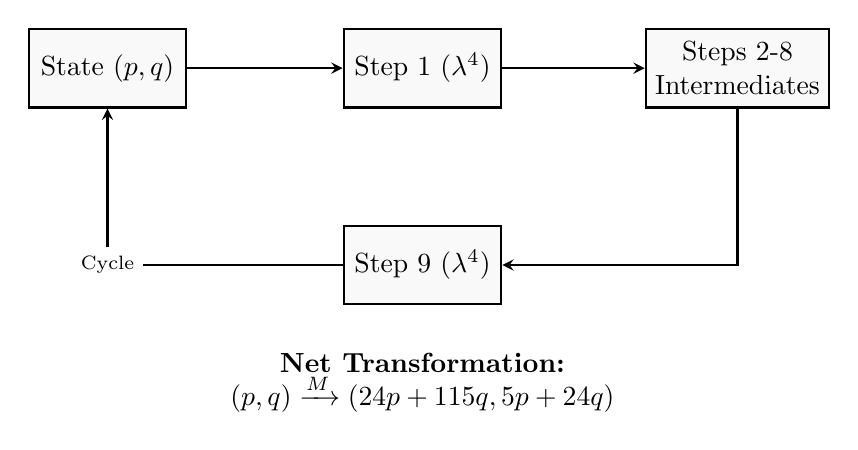
\begin{tikzpicture}[scale=1.0, every node/.style={transform shape}]
    % Styles
    \tikzstyle{state} = [rectangle, draw=black, thick, minimum width=2.0cm, minimum height=1cm, align=center, fill=gray!5]
    \tikzstyle{arrow} = [->, >=stealth, thick]
    \tikzstyle{label} = [midway, fill=white, font=\scriptsize]

    % Nodes - Abstracted for length
    \node[state] (S1) at (0, 0) {State $(p, q)$};
    \node[state] (S2) at (4, 0) {Step 1 ($\lambda^4$)};
    \node[state] (S3) at (8, 0) {Steps 2-8\\Intermediates};
    \node[state] (S4) at (4, -2.5) {Step 9 ($\lambda^4$)};

    % Arrows
    \draw[arrow] (S1) -- (S2);
    \draw[arrow] (S2) -- (S3);
    \draw[arrow] (S3) |- (S4);
    \draw[arrow] (S4) -| node[label] {Cycle} (S1);
    
    % Matrix annotation
    \node[draw=none, align=center] at (4, -4) {\textbf{Net Transformation:}\\ $(p, q) \xrightarrow{M} (24p+115q, 5p+24q)$};
\end{tikzpicture}
\end{center}

\subsection{Commentary}
The derivation for $\sqrt{23}$ illustrates the generality of the symmetric palindrome method. By constructing the operator sequence from the coefficients $[4, 1, 3, 1, 4]$, we generate the matrix corresponding to the fundamental Pell solution $(24, 5)$, ensuring exact convergence to $\sqrt{23}$.


\section{Detailed Factorization of $M'$}

The net transformation $M'$ for the Silver Ratio cycle is realized by a sequence of mediant and reciprocal operations. The matrix $M'$ is defined as $M' = \begin{pmatrix} -2 & 1 \\ 1 & 0 \end{pmatrix}$. The factorization $M' = SU(1)SU(1)SU(1)S$ is verified by direct multiplication:
\begin{align*}
SU(1) &= \begin{pmatrix} 0 & 1 \\ 1 & 0 \end{pmatrix} \begin{pmatrix} 1 & 1 \\ 0 & 1 \end{pmatrix} = \begin{pmatrix} 0 & 1 \\ 1 & 1 \end{pmatrix} \\
SU(1)S &= \begin{pmatrix} 0 & 1 \\ 1 & 1 \end{pmatrix} \begin{pmatrix} 0 & 1 \\ 1 & 0 \end{pmatrix} = \begin{pmatrix} 1 & 0 \\ 1 & 1 \end{pmatrix} \\
SU(1)SU(1) &= \begin{pmatrix} 1 & 0 \\ 1 & 1 \end{pmatrix} \begin{pmatrix} 1 & 1 \\ 0 & 1 \end{pmatrix} = \begin{pmatrix} 1 & 1 \\ 1 & 2 \end{pmatrix} \\
SU(1)SU(1)S &= \begin{pmatrix} 1 & 1 \\ 1 & 2 \end{pmatrix} \begin{pmatrix} 0 & 1 \\ 1 & 0 \end{pmatrix} = \begin{pmatrix} 1 & 1 \\ 2 & 1 \end{pmatrix} \\
SU(1)SU(1)SU(1) &= \begin{pmatrix} 1 & 1 \\ 2 & 1 \end{pmatrix} \begin{pmatrix} 1 & 1 \\ 0 & 1 \end{pmatrix} = \begin{pmatrix} 1 & 2 \\ 2 & 3 \end{pmatrix} \\
SU(1)SU(1)SU(1)S &= \begin{pmatrix} 1 & 2 \\ 2 & 3 \end{pmatrix} \begin{pmatrix} 0 & 1 \\ 1 & 0 \end{pmatrix} = \begin{pmatrix} 2 & 1 \\ 3 & 2 \end{pmatrix}
\end{align*}
The sequence of operations is: 1. Swap. 2. Mediant (i.e., apply U(1)). 3. Swap. 4. Mediant. 5. Swap. 6. Mediant. 7. Swap. 8. Mediant. This sequence of eight steps yields the net transformation $M'$. We call this an extended triadic cycle.

\section{Worked Example}

We demonstrate the triadic recurrence trajectory for an initial state $(p_0, q_0) = (3, 2)$. The associated rational value is $R_0 = 3/2 = 1.5$. The triadic cycle operates in three phases: Emission, Memory, and Return.

\begin{enumerate}
    \item **Initial State:** $(p_0, q_0) = (3, 2)$. Ratio $R_0 = 1.5$.
    \item **Phase 0 (Emission):** Apply $(p, q) \rightarrow (p + q, p)$. The state transitions to $(p_1, q_1) = (3 + 2, 3) = (5, 3)$. Ratio $R_1 = 5/3 \approx 1.667$.
    \item **Phase 1 (Memory):** Apply $(p, q) \rightarrow (p + q, p)$. The state transitions to $(p_2, q_2) = (5 + 3, 5) = (8, 5)$. Ratio $R_2 = 8/5 = 1.6$.
    \item **Phase 2 (Return):** Apply $(p, q) \rightarrow (q, p)$. The state transitions to $(p_3, q_3) = (5, 8)$. Ratio $R_3 = 5/8 = 0.625$.
\end{enumerate}
The first full cycle results in the state $(5, 8)$. The next cycle begins with this state. The sequence converges to the limits $1/\sqrt{2}$, $1 + \sqrt{2}$, and $\sqrt{2}$ alternately.

\section{General Construction Template}

The general construction template for a quadratic irrational $\alpha$ satisfying $\alpha^2 - T\alpha + D = 0$ involves decomposing the target matrix $M_\alpha = \begin{pmatrix} a & b \\ c & d \end{pmatrix}$ into elementary matrices $U(k) = \begin{pmatrix} 1 & k \\ 0 & 1 \end{pmatrix}$ and $S = \begin{pmatrix} 0 & 1 \\ 1 & 0 \end{pmatrix}$. The procedure is as follows:

\begin{enumerate}
    \item **Target Matrix Selection:** Identify the target matrix $M_\alpha$ corresponding to the quadratic irrational $\alpha$. The matrix must satisfy $a + d = T$ and $ad - bc = D$.
    \item **Decomposition Algorithm:** Determine the integers $k_1, k_2, k_3$ from the matrix components using the integer-only algorithm derived in Section 9.2. The key equations are $k_2 = c$, $k_1 = (d - 1)/c$, and $k_3 = (a - 1)/c$.
    \item **Operator Sequence Generation:** Construct the triadic cycle by mapping each $U(k_i)$ to $k_i$ mediant operations and each $S$ to a reciprocal operation. The sequence of operations is then applied iteratively to generate the rational approximation sequence.
\end{enumerate}

\section{Extended Commentary}

The framework's core principle of structural integrity ensures that all information, including the history of arithmetic operations, is preserved within the state itself. This approach allows for the simulation of complex physical phenomena, where irrationality emerges as a statistical artifact of high-frequency rational oscillation, rather than an ontological primitive. The framework's capacity to model these physical phenomena suggests that the proposed non-event axiom provides a consistent foundation for further development.

\end{document}